\chapter{War}

\begin{figure}[H]
   \centering
   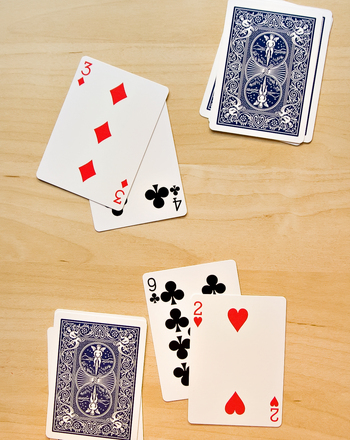
\includegraphics[width=1.0\linewidth,height=0.5\linewidth]{fig100001.png}
   \caption{"War" \\ https://images.squarespace-cdn.com/content/v1/59ea6080a803bb2f70ecbae5/1529350057743-92YH5Y0BN0JUMYB6X7NV/close-call-slide.jpg}
\label{fig100001}
\end{figure}

The game "War" (Fig. \ref{fig100001}) is a children's card game, and in its basic version, it is played by two players. The cards are standard, 52 playing cards. Card suits are equal, and there is no power per suit. Each card has a power with which it participates in the game, starting with the pairs (2 points) and going up to the aces (14 points). The deck of cards is shuffled and dealt equally to both players. The cards are dealt face down, with each player showing the top card on each turn. The player with the stronger card takes both cards. If the cards are of equal strength, it is a "war," and the players show three cards each. The war is won by the player with the stronger third card. If the third cards also match, the war continues until one player loses the war. The winning player collects all face-up cards. Draw cards always go to the bottom of the respective player's deck. The game is lost by that player who runs out of cards.

\section{Designing the GUI}

The game is relatively simple and does not require special skills, which makes it an ideal option for young children. Developing this game as a mobile application begins with creating a new project (Fig. \ref{fig100002}).

\begin{figure}[H]
   \centering
   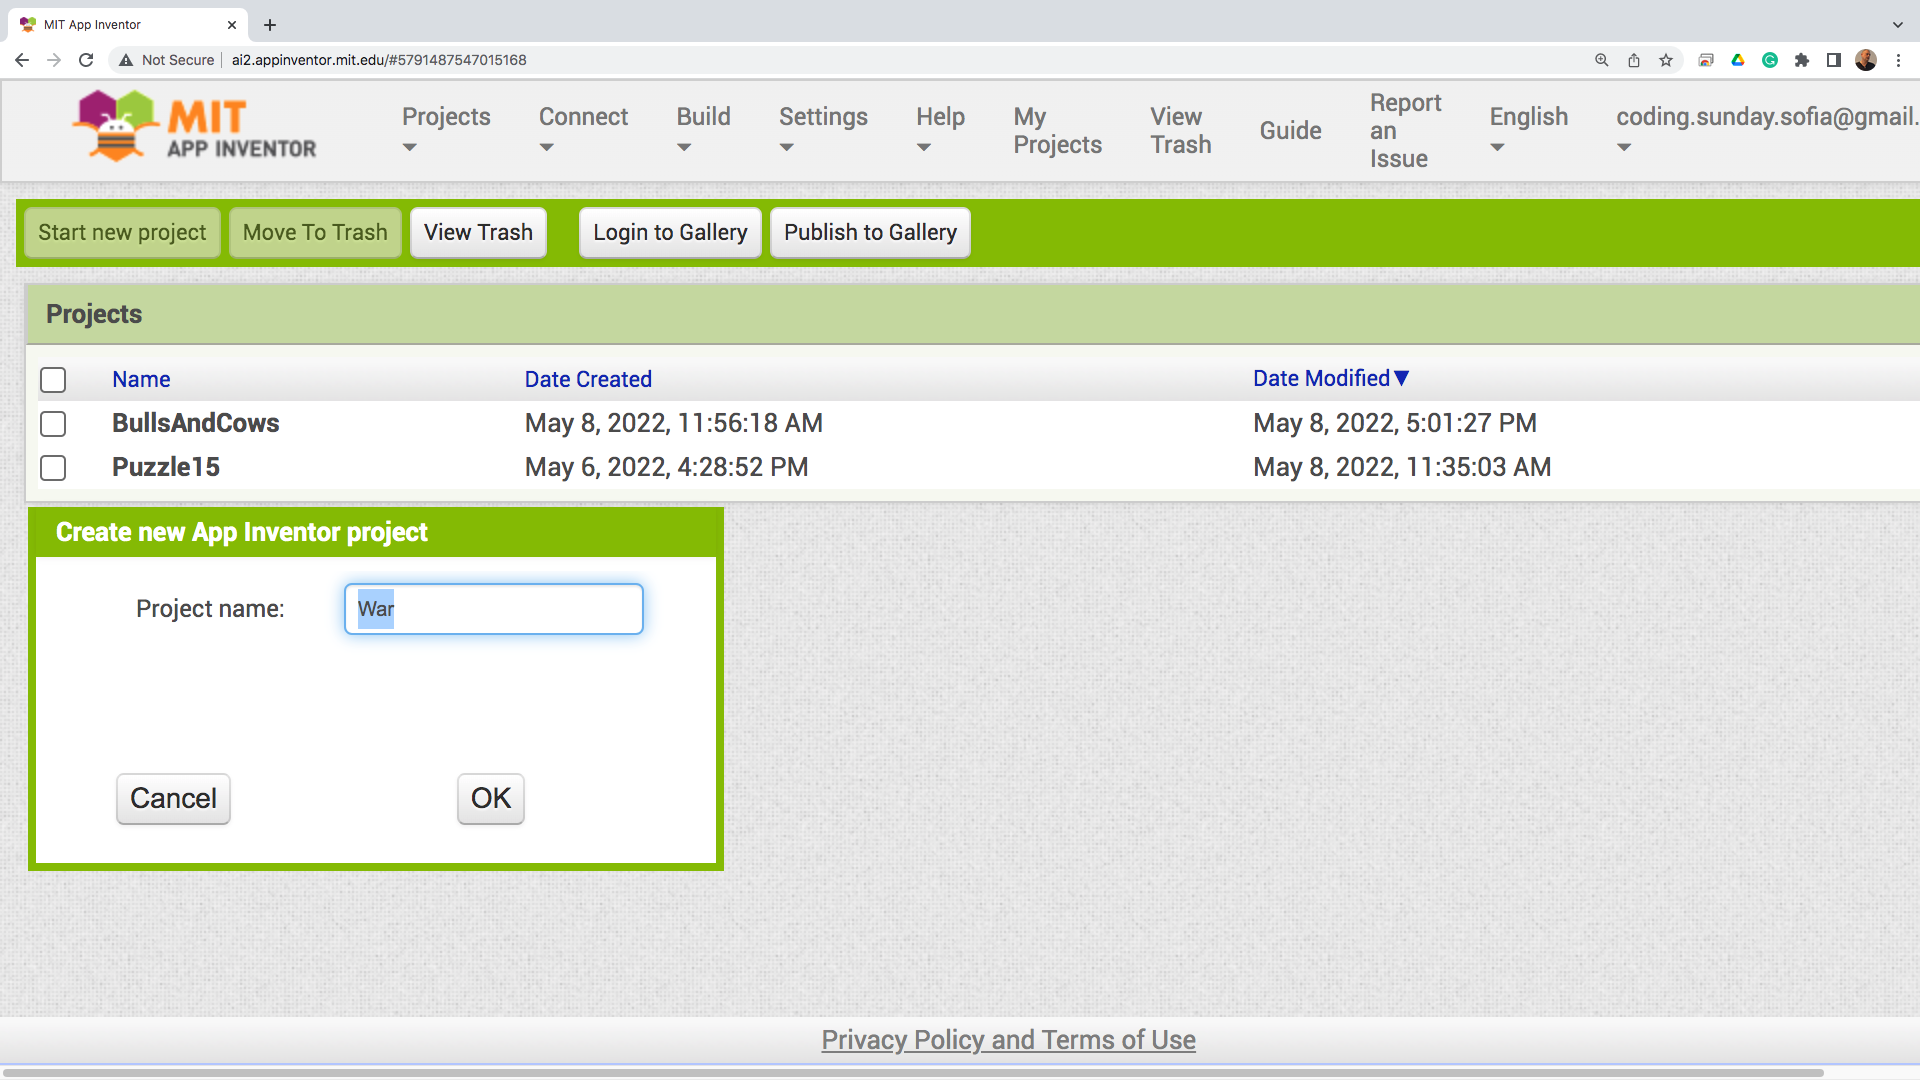
\includegraphics[width=1.0\linewidth,height=0.5\linewidth]{fig100002.png}
   \caption{Creating a new War game project}
\label{fig100002}
\end{figure}

The user interface will be as simple as possible. Two buttons (Fig. \ref{fig100003}) at the workspace will start a new game and make a move.

\begin{figure}[H]
   \centering
   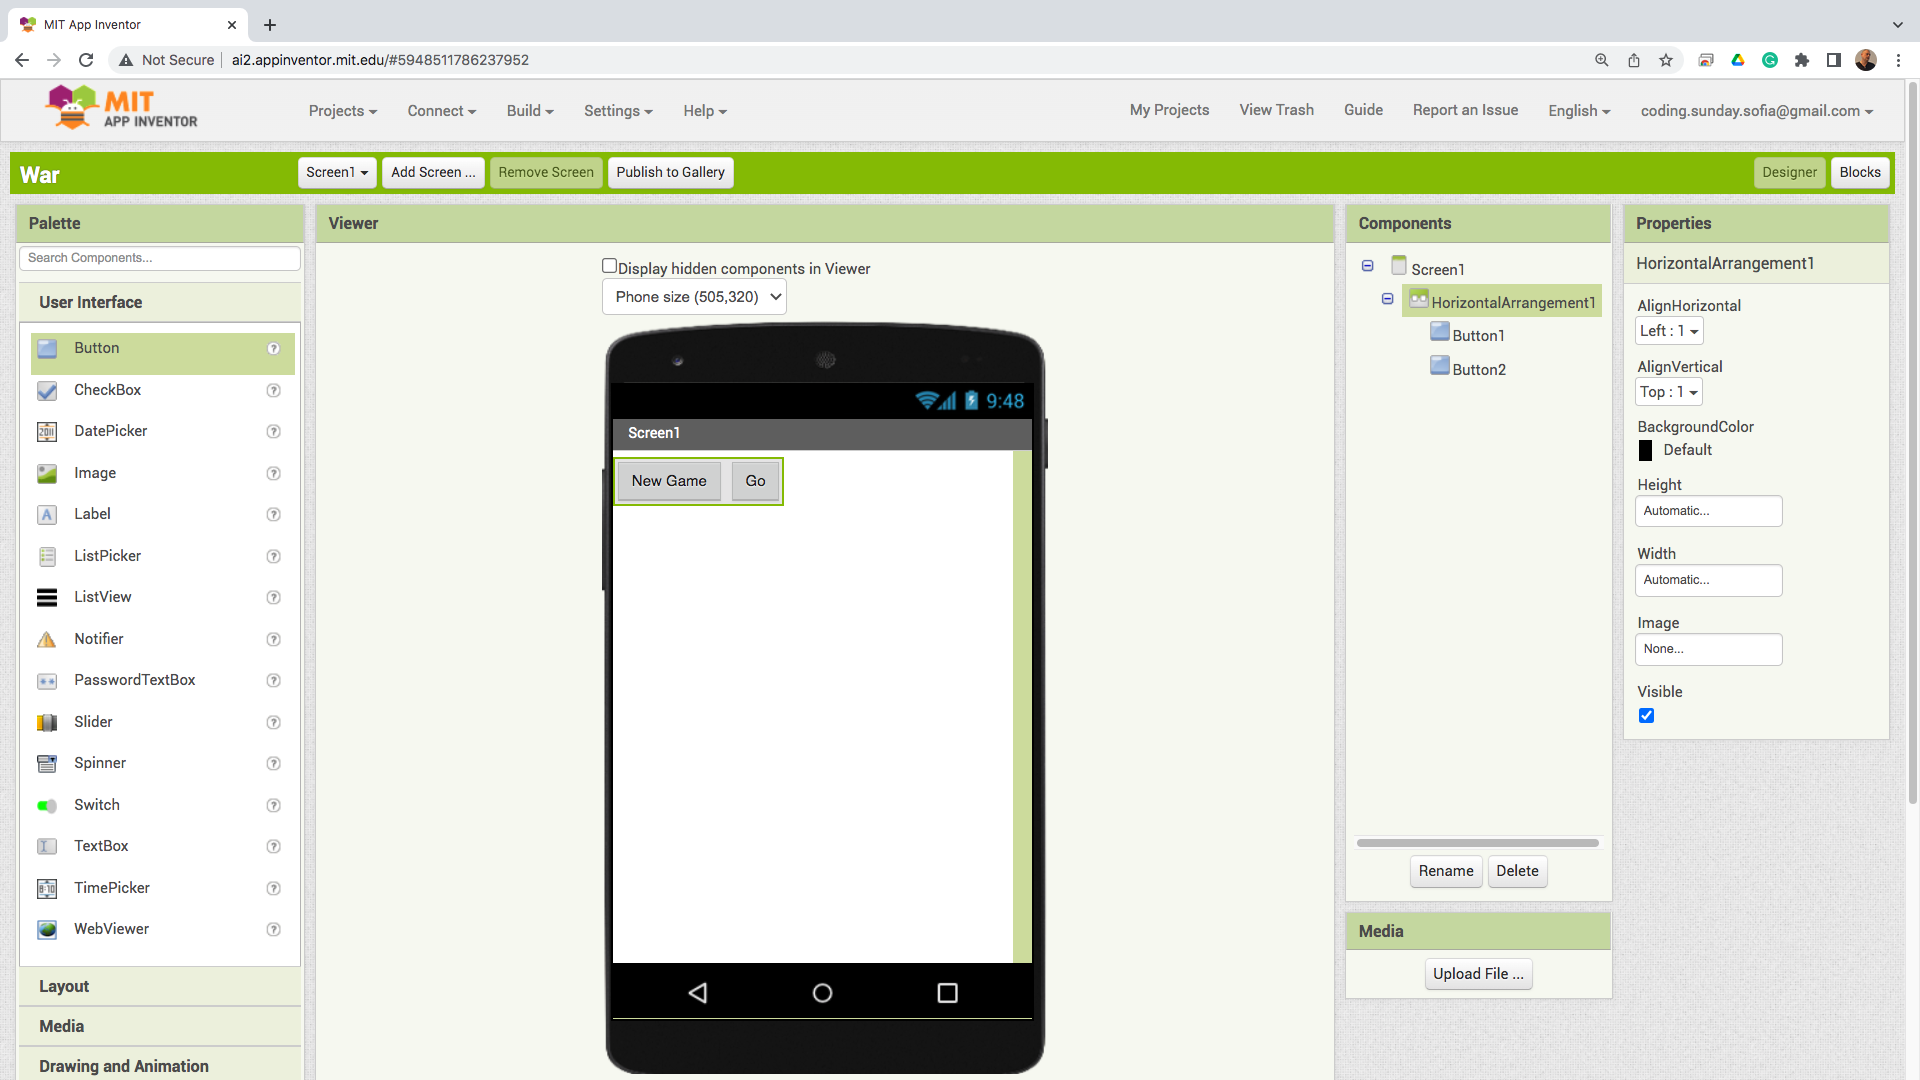
\includegraphics[width=1.0\linewidth,height=0.5\linewidth]{fig100003.png}
   \caption{Start New Game and Make Move Buttons}
\label{fig100003}
\end{figure}

Immediately below the buttons, two rows of visual components for displaying graphic images are arranged in tabular form (Fig. \ref{fig100004}). The first column will show a card back, which symbolizes the decks of both players, and the other three adjacent components will display one card when there is no war and three cards when there is a war.

\begin{figure}[H]
   \centering
   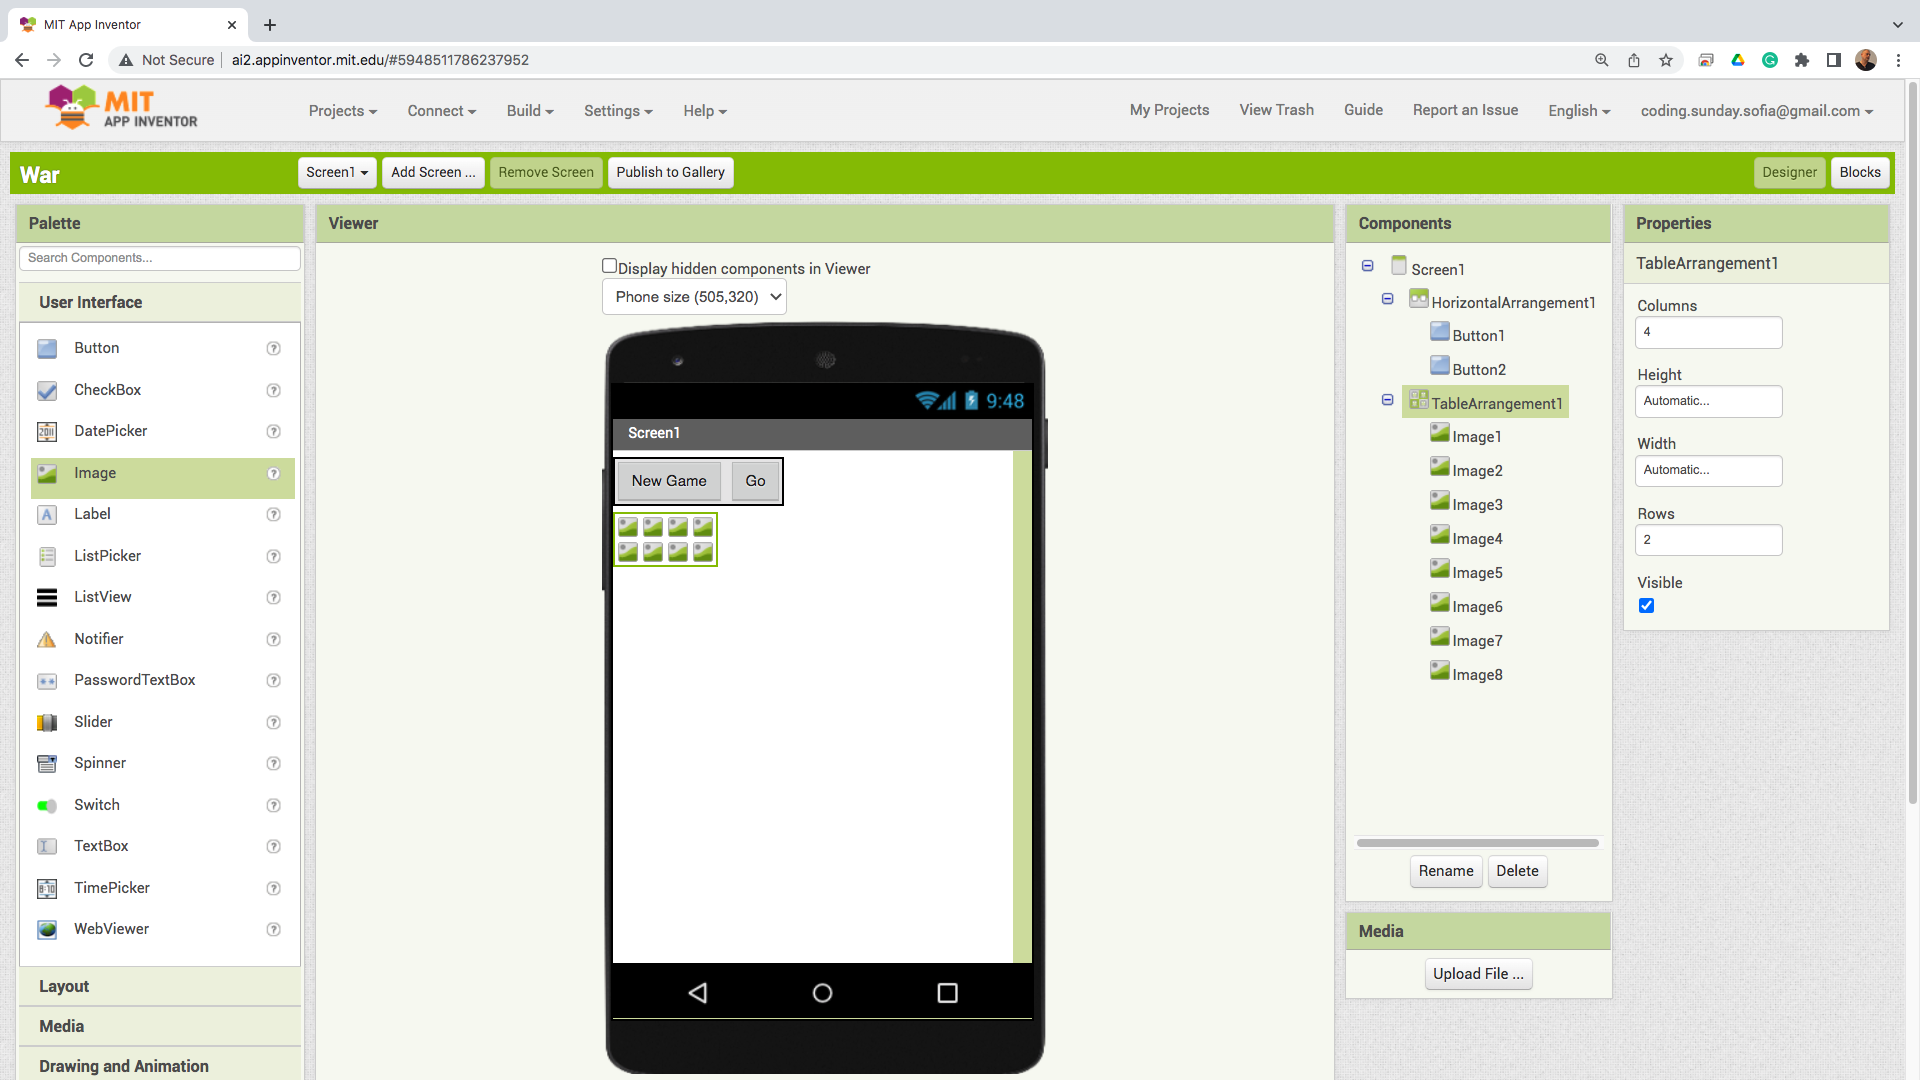
\includegraphics[width=1.0\linewidth,height=0.5\linewidth]{fig100004.png}
   \caption{Map Visualization Components}
\label{fig100004}
\end{figure}

For the map images, any set of maps distributed under a free license for non-commercial use can be used (Fig. \ref{fig100005}).

\begin{figure}[H]
   \centering
   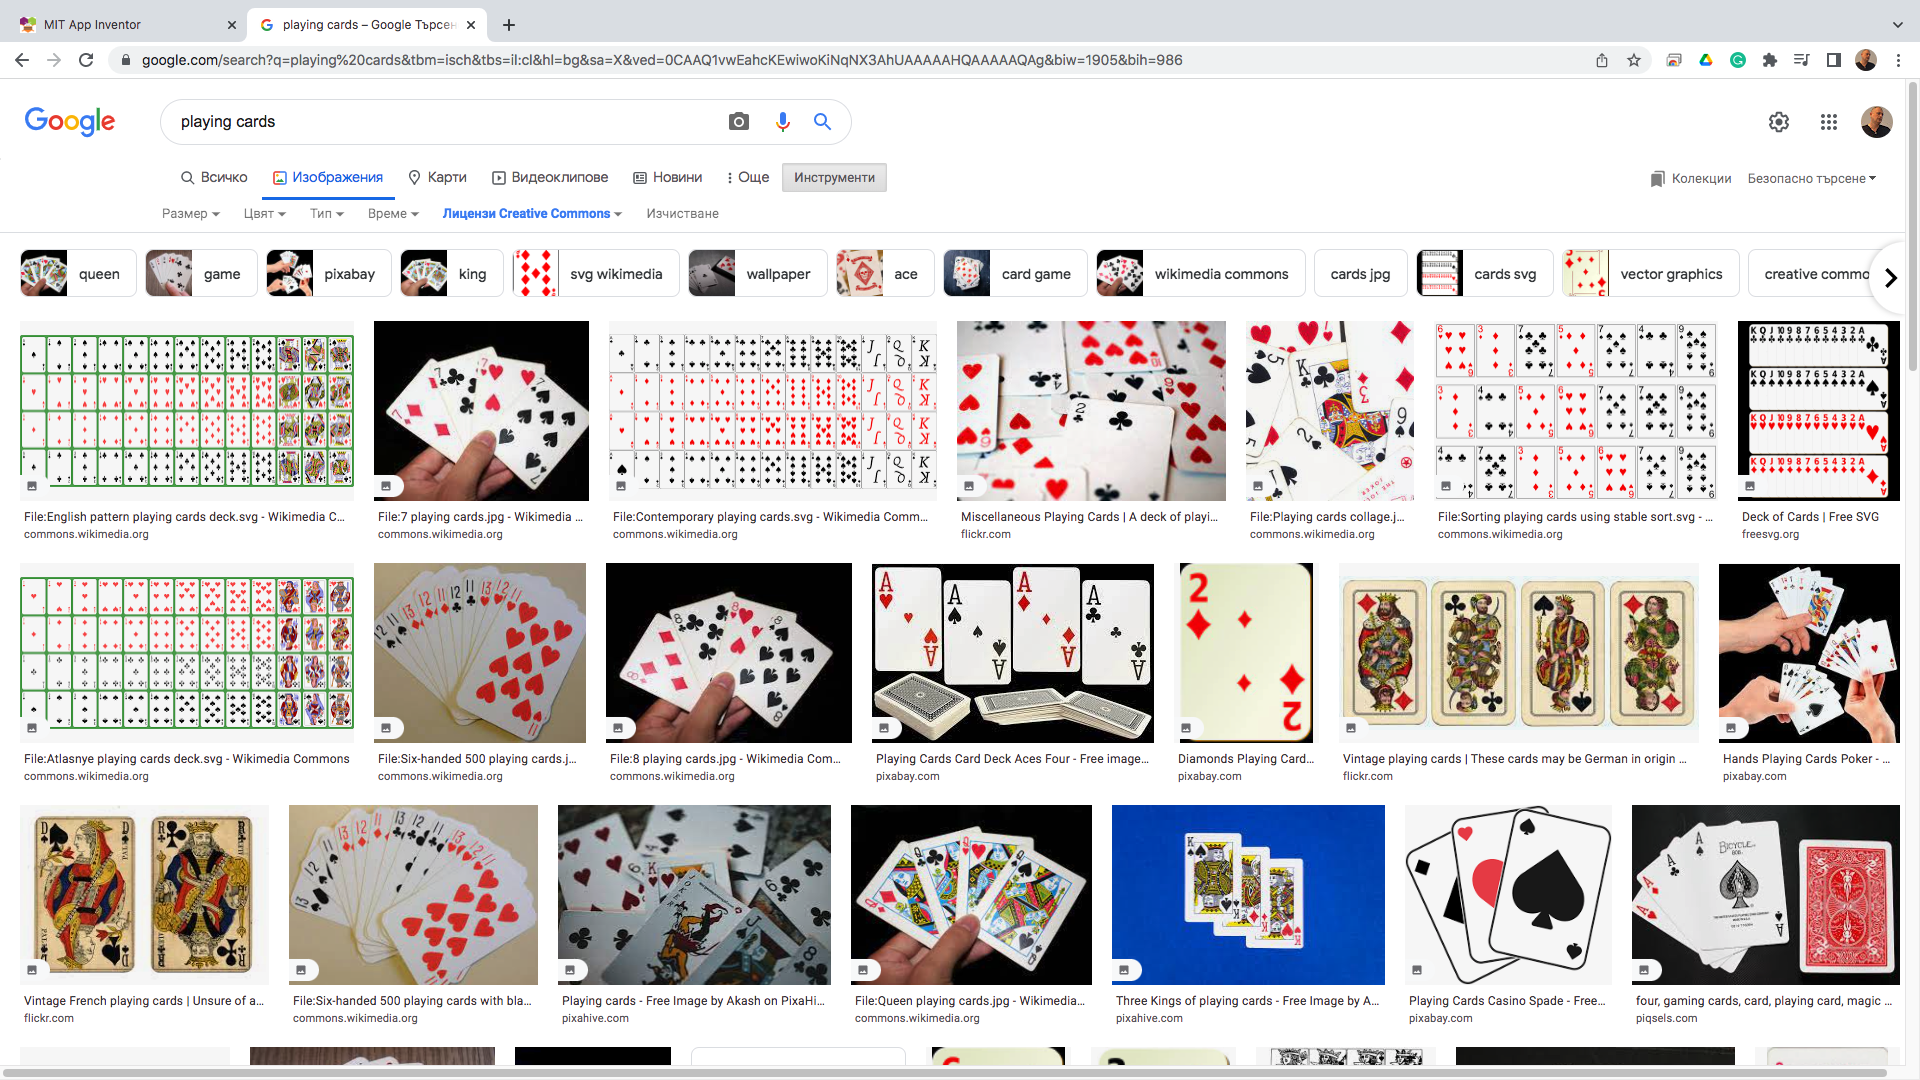
\includegraphics[width=1.0\linewidth,height=0.5\linewidth]{fig100005.png}
   \caption{Images of playing cards}
\label{fig100005}
\end{figure}

If the card set is in a common image, it is cut into 52 separate images and at least one card back image. The 53 graphic files thus prepared are loaded into the project by uploading file by file (Fig. \ref{fig100006}).

\begin{figure}[H]
   \centering
   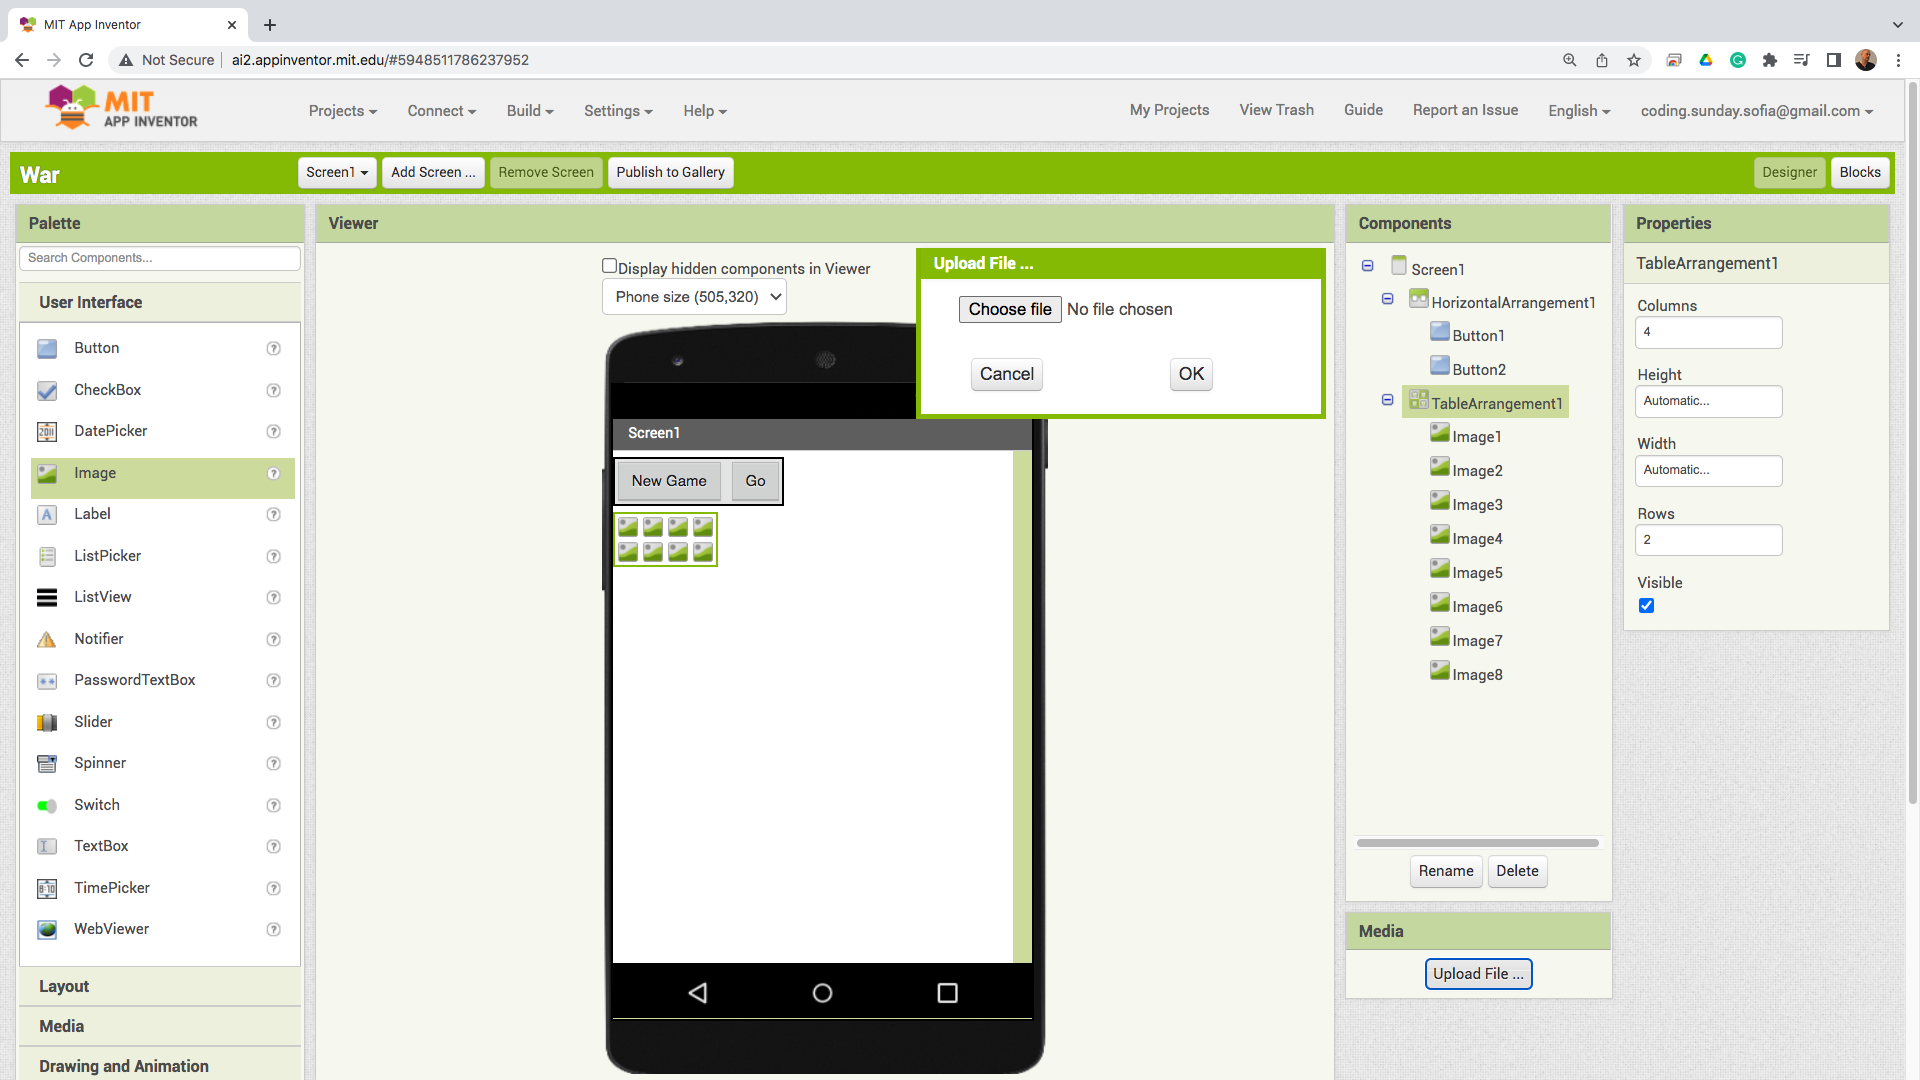
\includegraphics[width=1.0\linewidth,height=0.5\linewidth]{fig100006.png}
   \caption{Upload image files}
\label{fig100006}
\end{figure}

From the graphics files thus uploaded, the card back image is loaded into the first column of images (Fig. \ref{fig100007}).

\begin{figure}[H]
   \centering
   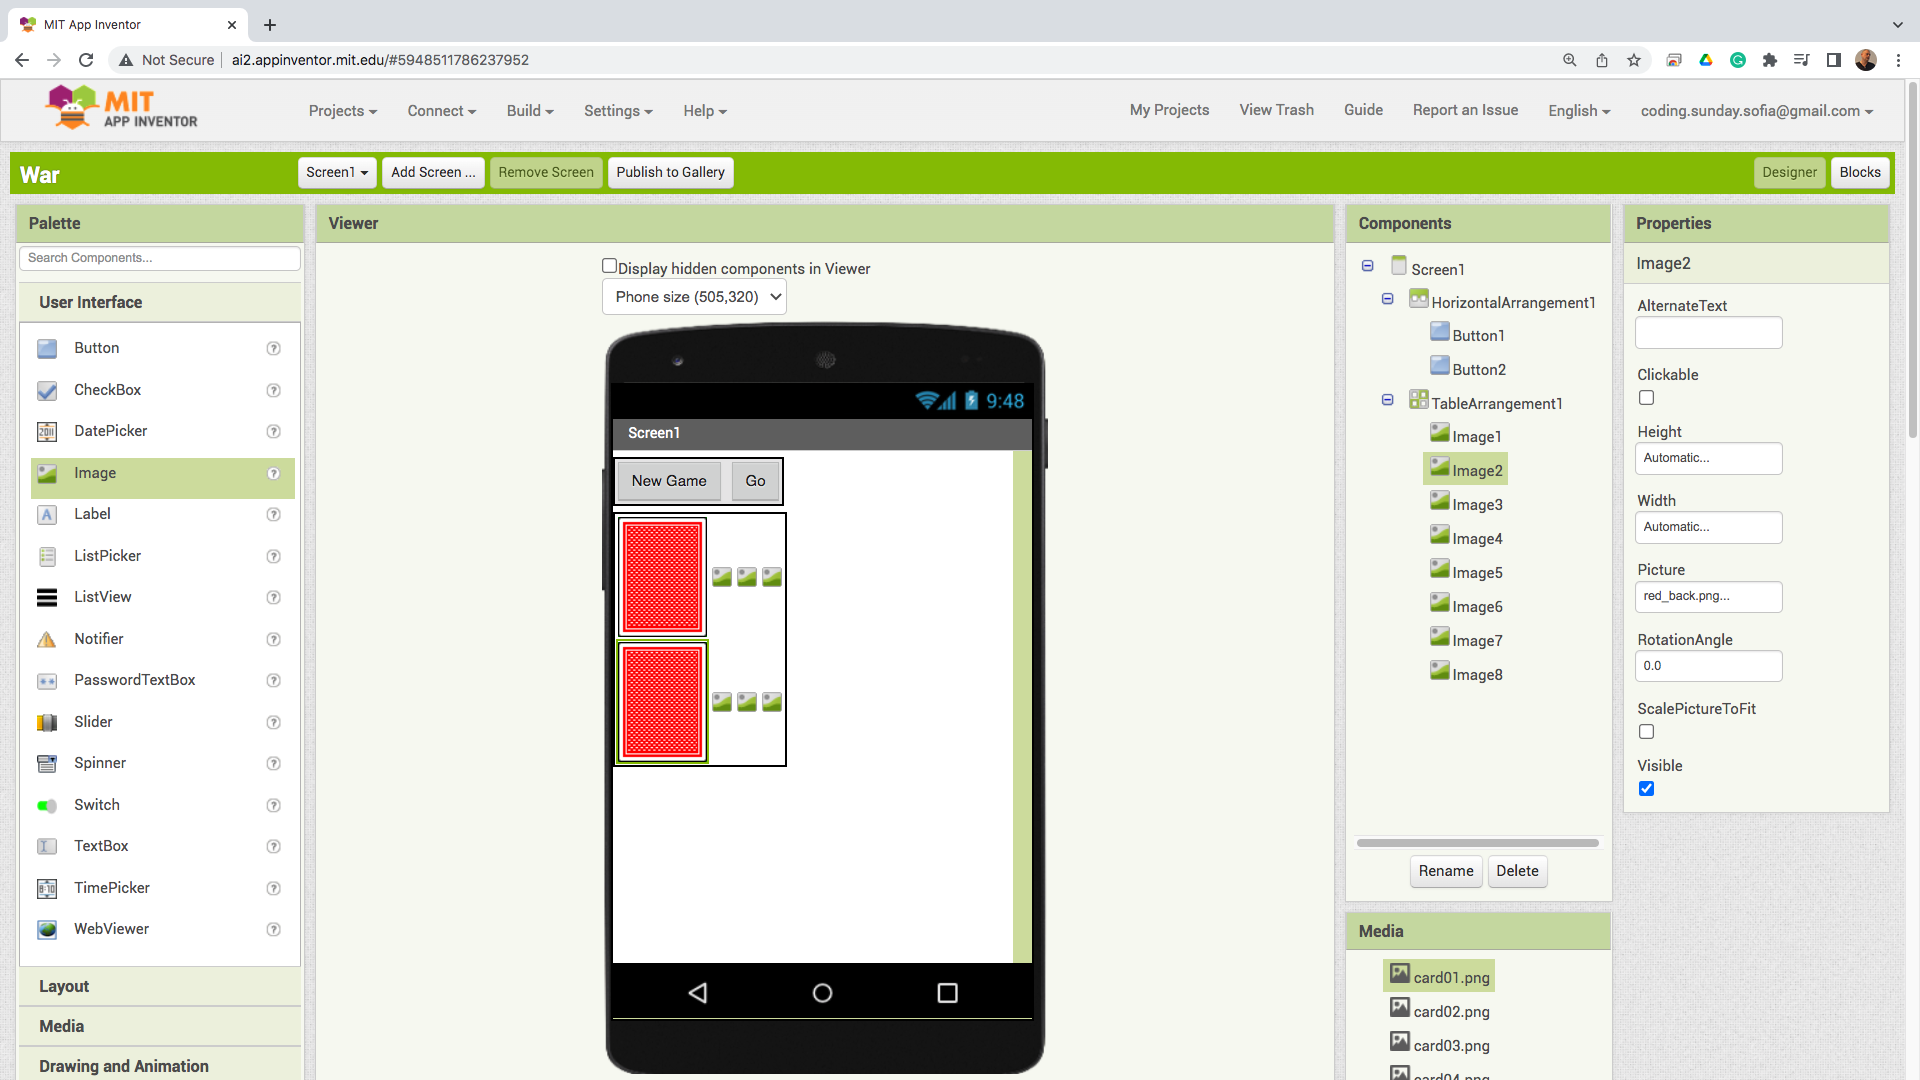
\includegraphics[width=1.0\linewidth,height=0.5\linewidth]{fig100007.png}
   \caption{Images for marking the decks}
\label{fig100007}
\end{figure}

\section{Using Data Structures}

Cards will circulate in the game model as integers. For this purpose, five auxiliary global variables are declared - a list of the main deck, two lists for the cards held by the player, and two lists for the cards placed on the table by the players (Fig. \ref{fig100008}).

\begin{figure}[H]
   \centering
   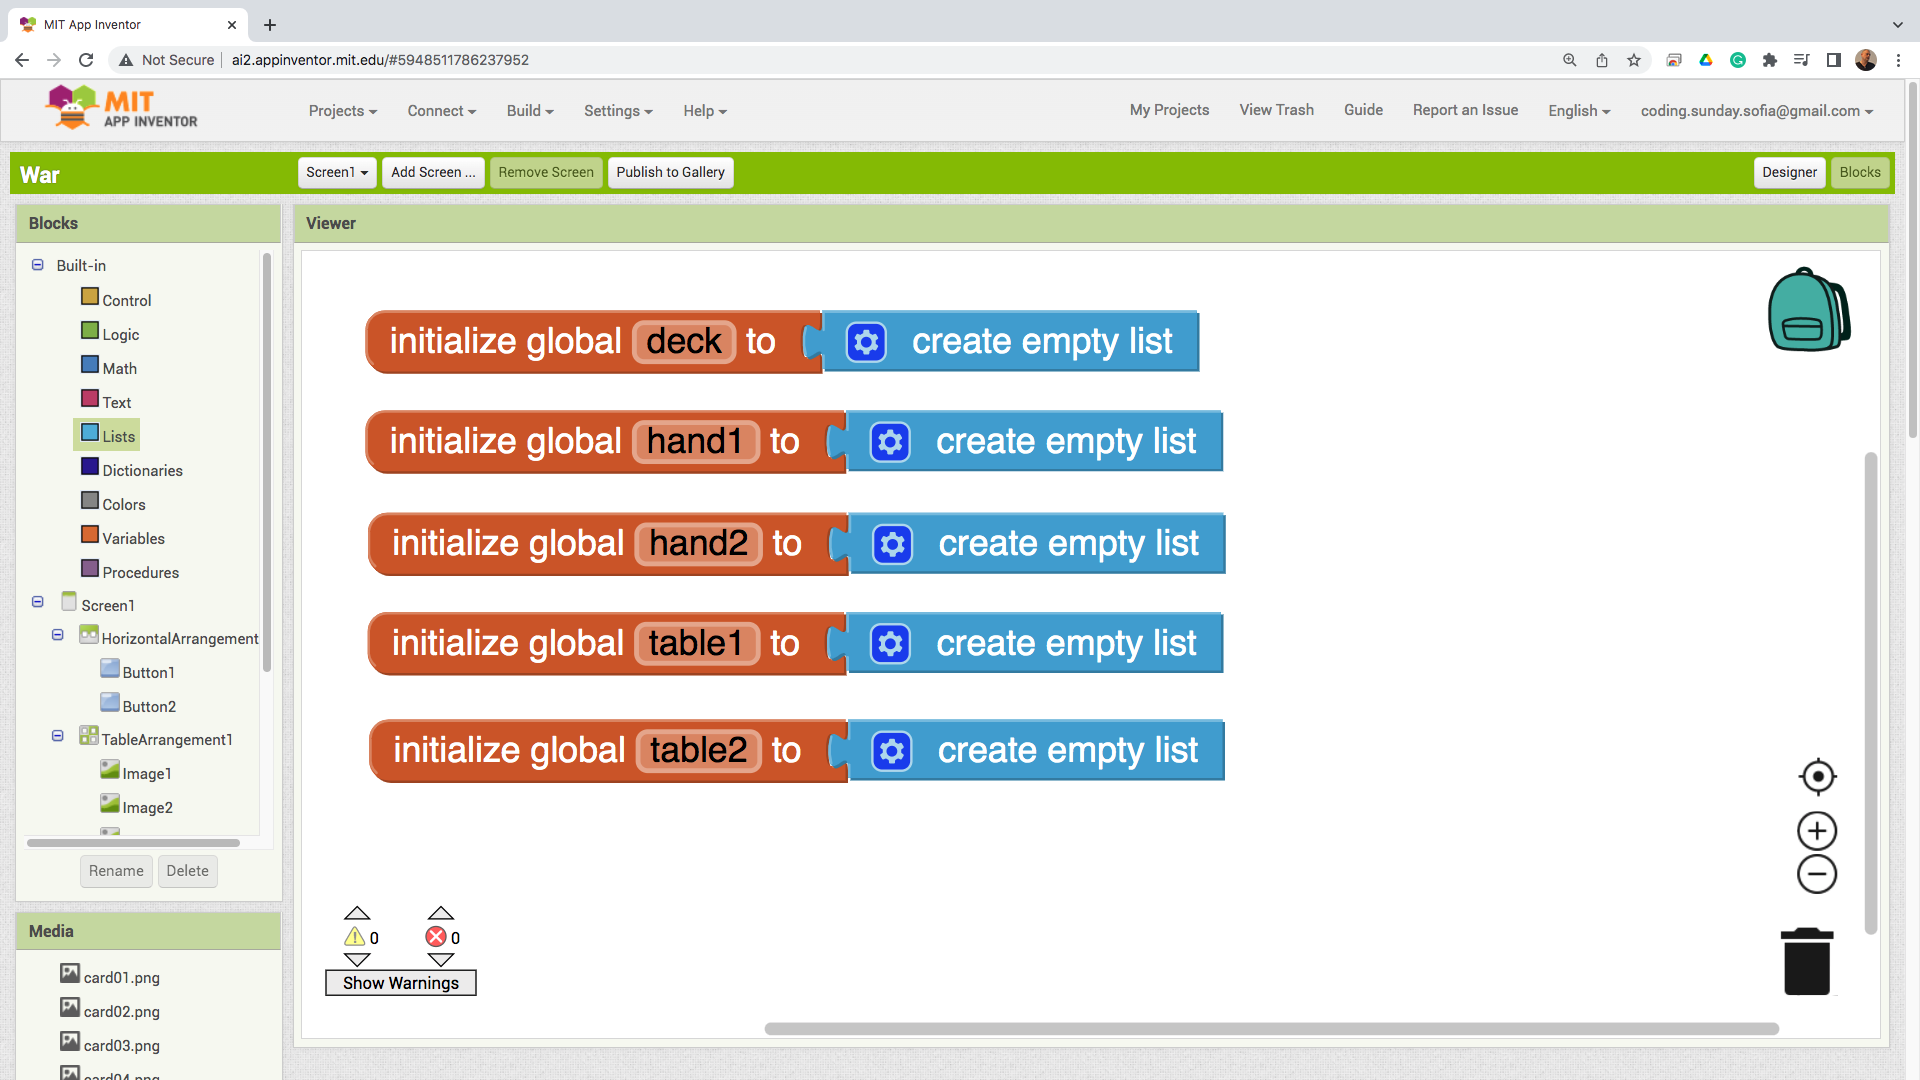
\includegraphics[width=1.0\linewidth,height=0.5\linewidth]{fig100008.png}
   \caption{Basic Auxiliary Variables}
\label{fig100008}
\end{figure}

Two additional lists make it easier to visualize the cards being placed on the table. These lists contain references to the visual components for displaying images (Fig. \ref{fig100009}).

\begin{figure}[H]
   \centering
   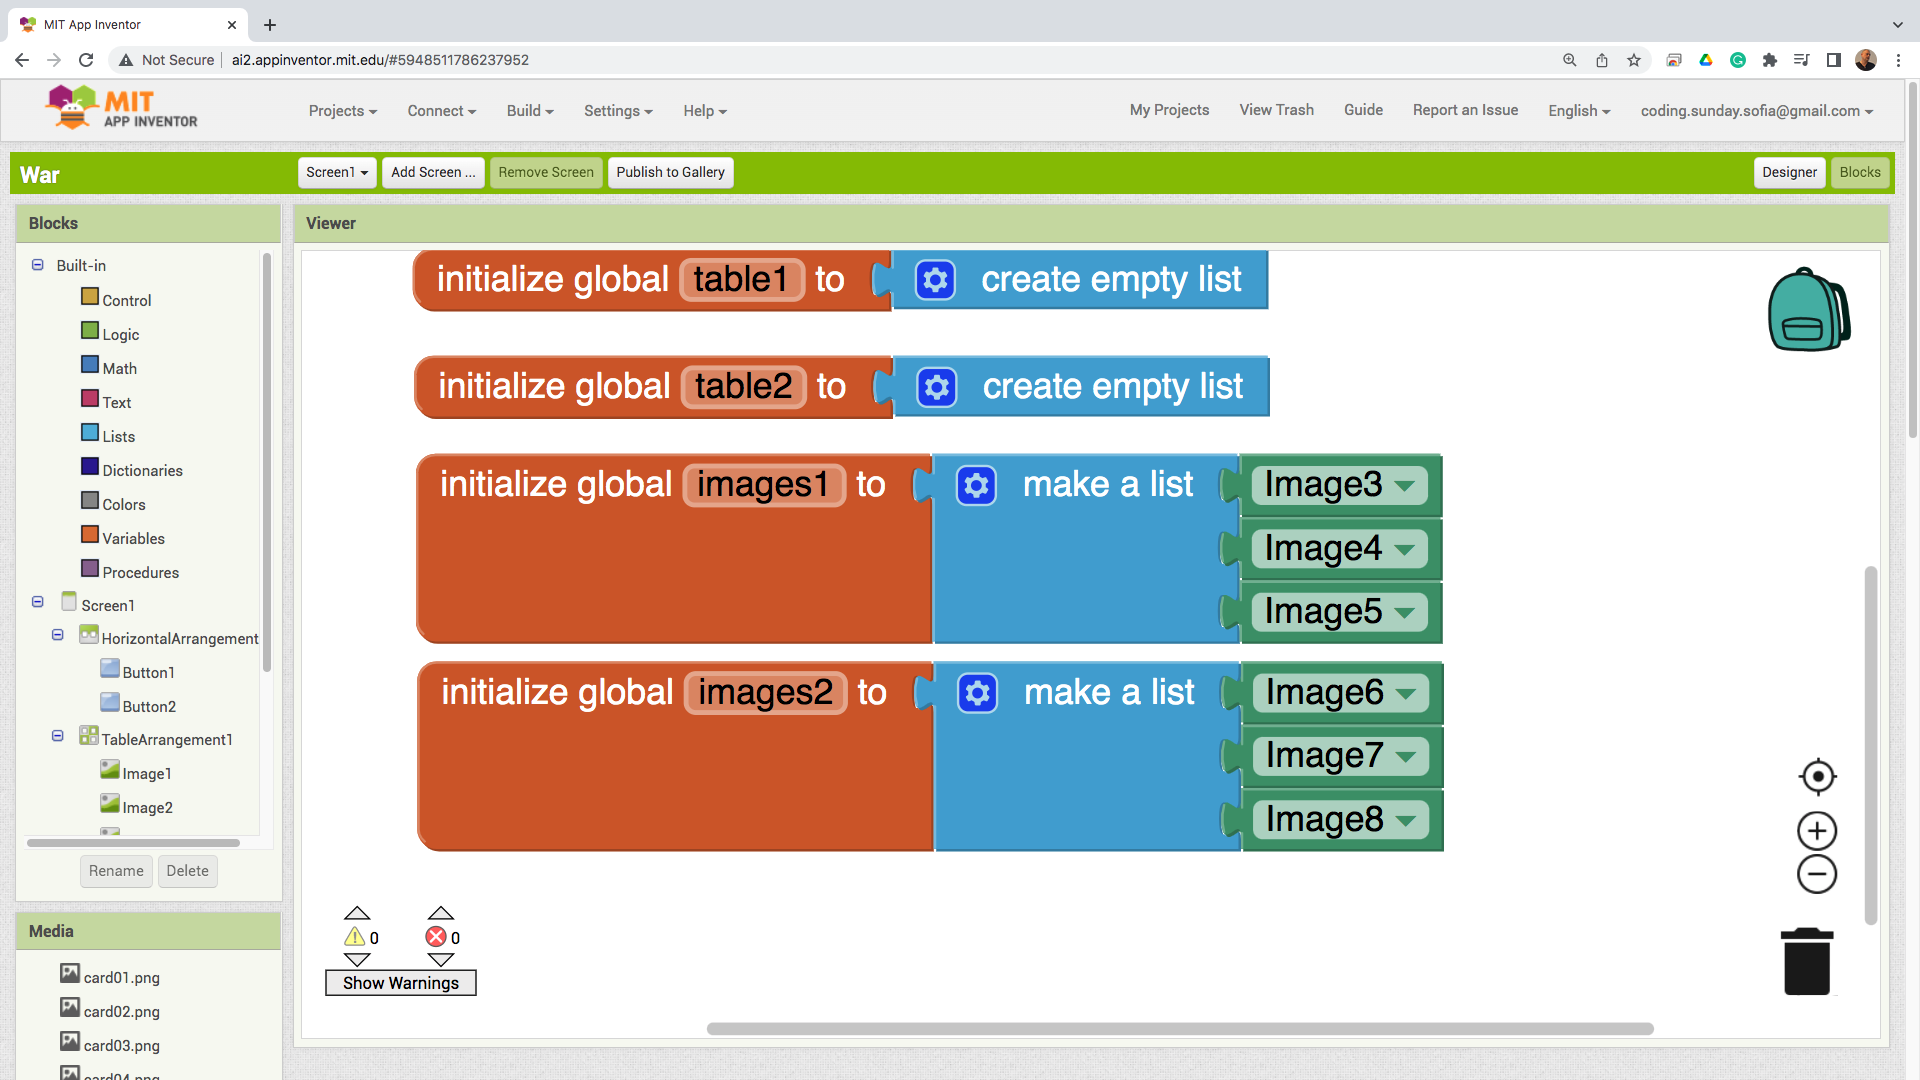
\includegraphics[width=1.0\linewidth,height=0.5\linewidth]{fig100009.png}
   \caption{Helper Visualization Lists}
\label{fig100009}
\end{figure}

The last helper variable trims the map images into a list. The order is essential, with deuces in the first four places, threes in the second four places, and so on until the last four places are aces (Fig. \ref{fig100010}). Thanks to this arrangement, the calculation of the winners in the individual rounds will be achieved by a simple arithmetic calculation.

\begin{figure}[H]
   \centering
   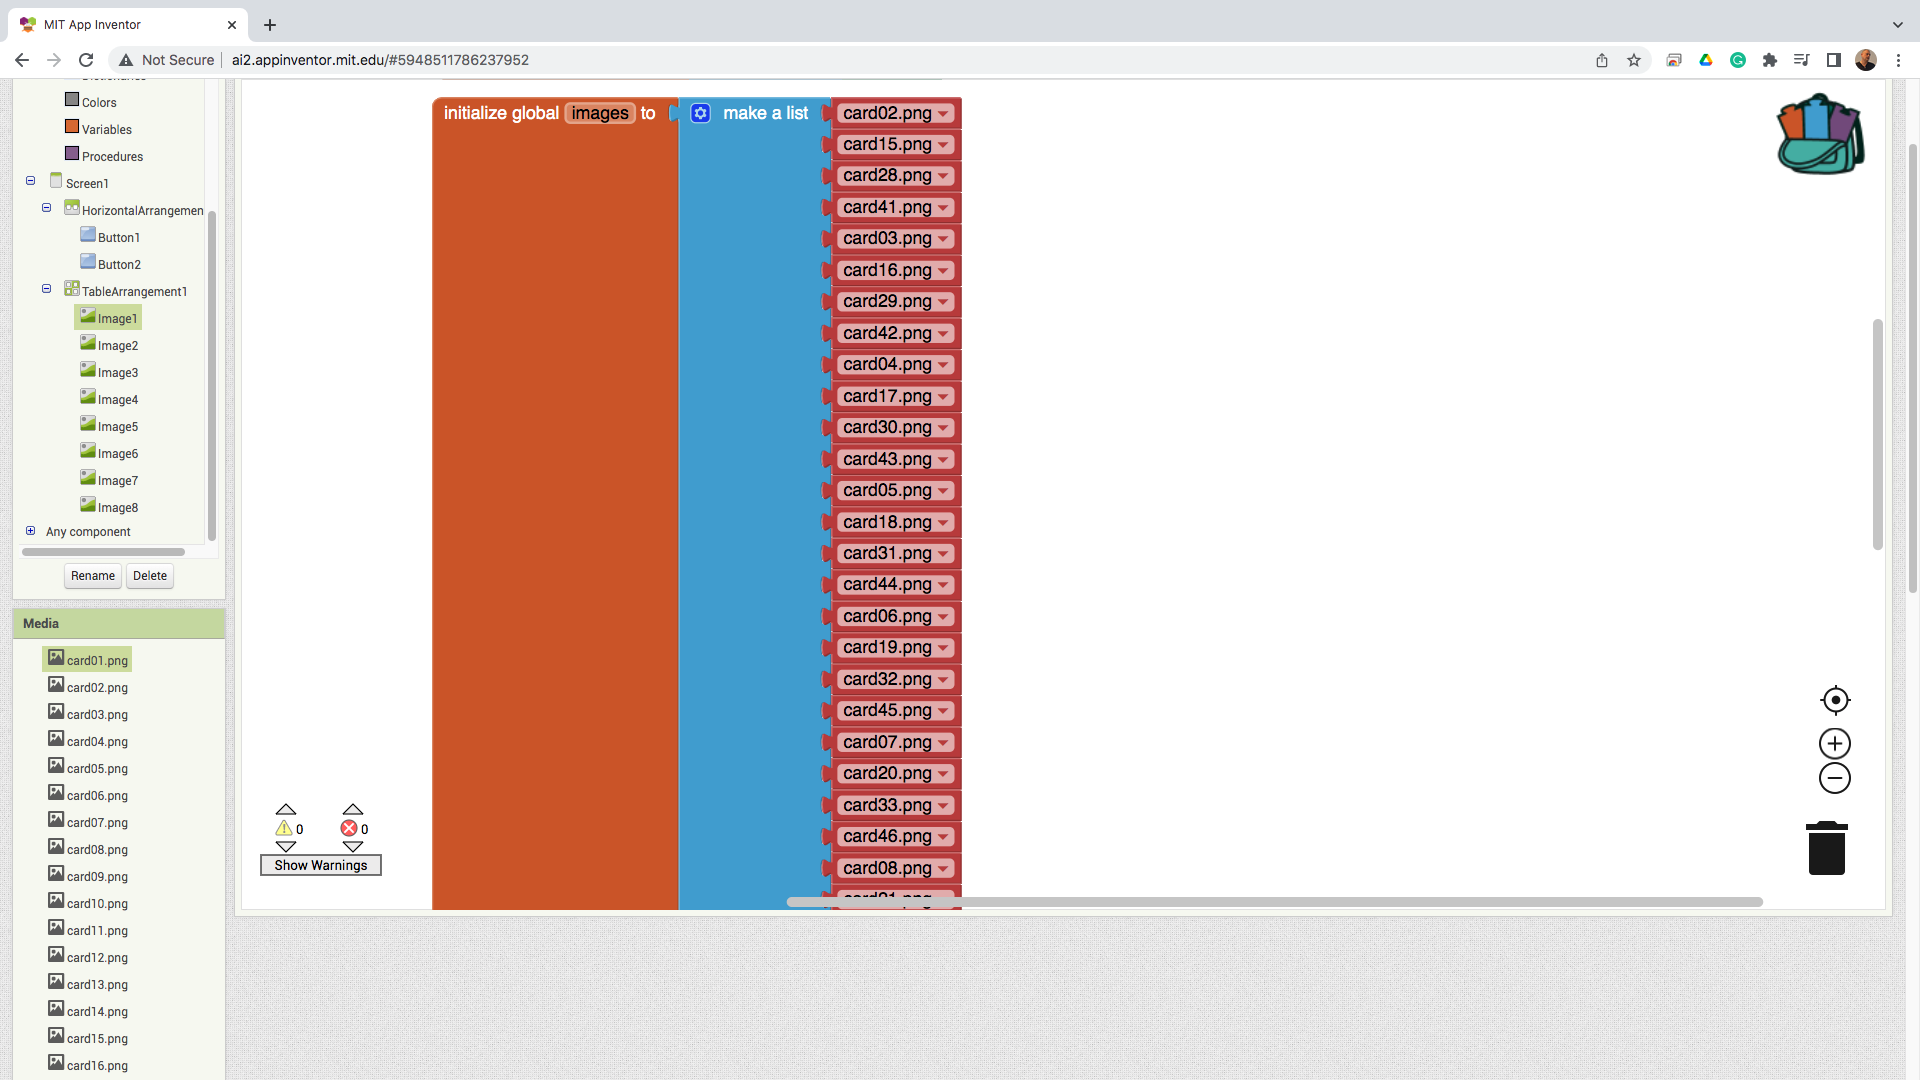
\includegraphics[width=1.0\linewidth,height=0.5\linewidth]{fig100010.png}
   \caption{Helper variable for order of cards by strength}
\label{fig100010}
\end{figure}

\section{Algorithms for manipulation of structures in the game}

Starting the game is all about organizing the individual lists correctly. To begin with, all auxiliary lists should be initialized with an empty value so that no parasitic information from previous plays is passed. A helper function can best achieve this (Fig. \ref{fig100011}).

\begin{figure}[H]
   \centering
   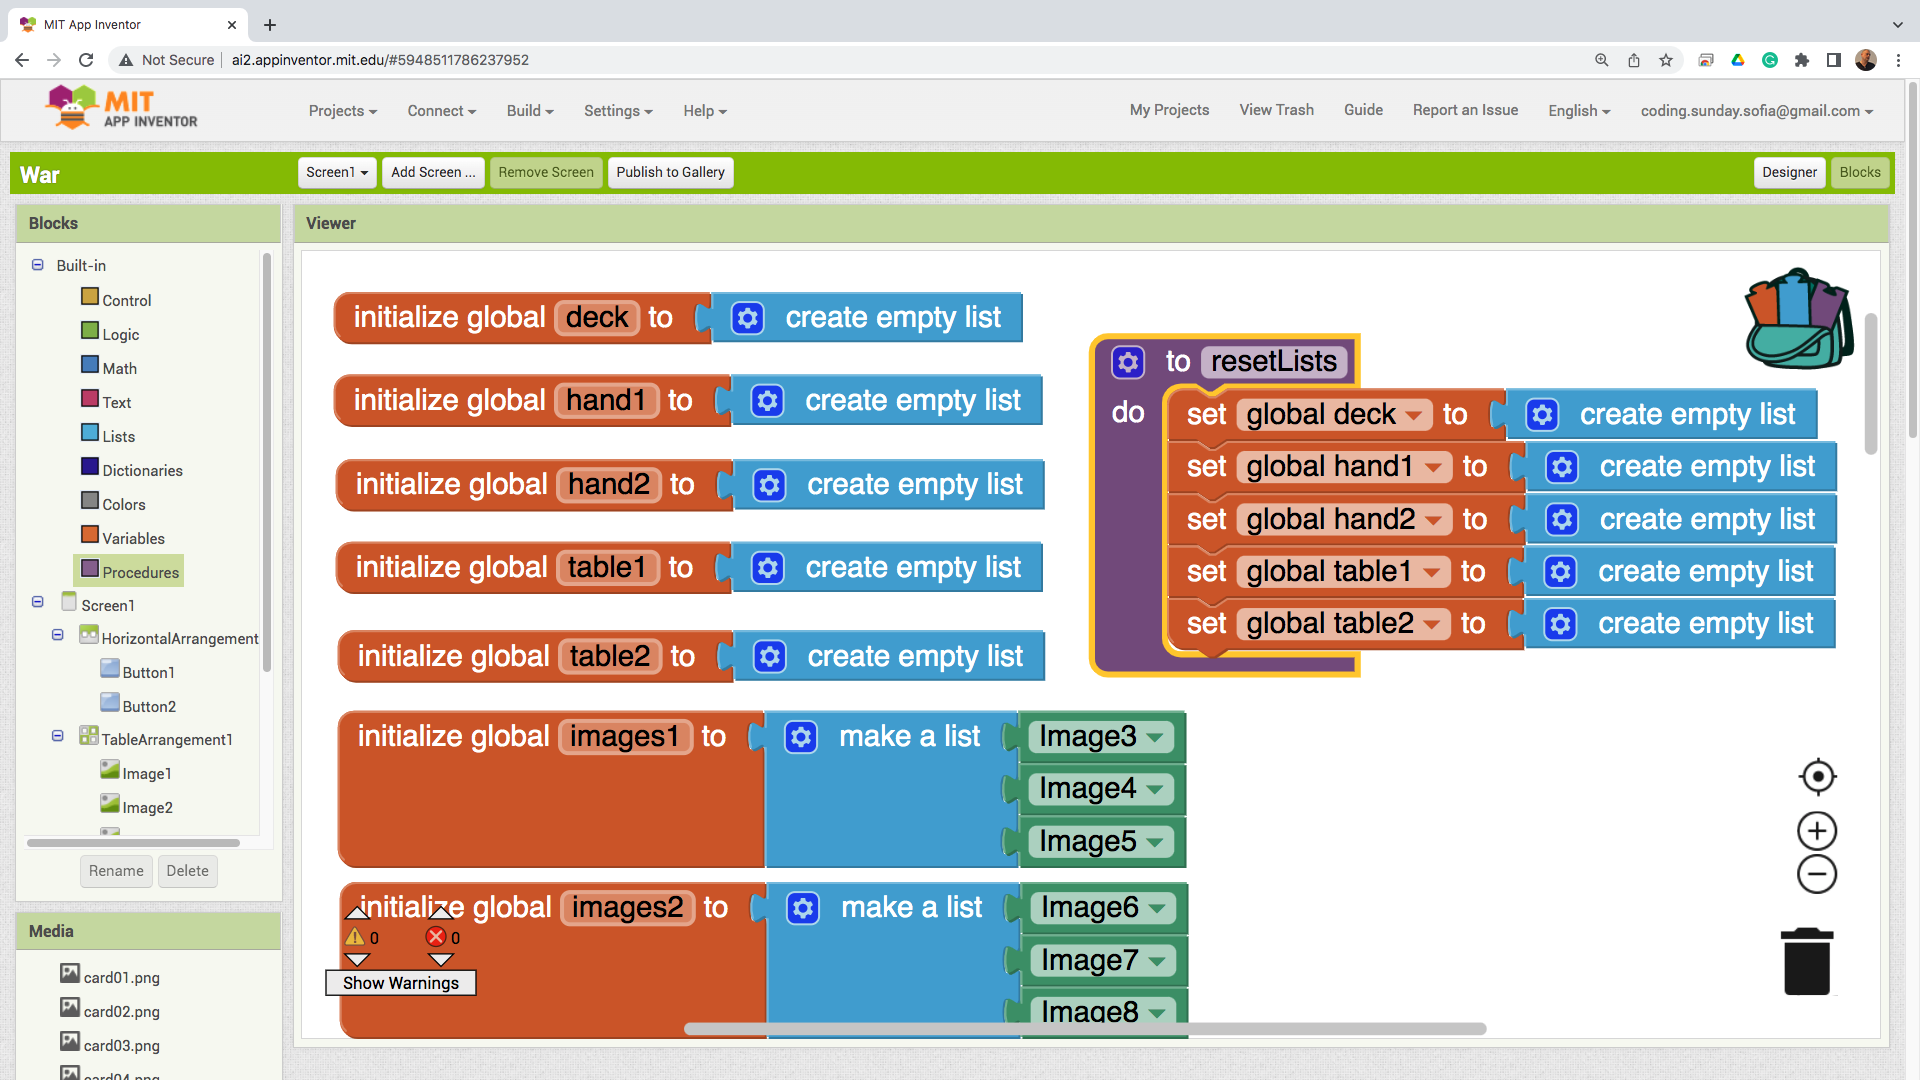
\includegraphics[width=1.0\linewidth,height=0.5\linewidth]{fig100011.png}
   \caption{Initialization of empty lists}
\label{fig100011}
\end{figure}

The main deck of cards contains, in a shuffled form, the numbers 1 to 52. Each number is the index of the corresponding card in the auxiliary list of card images. A loop is spun to populate the main deck (Fig. \ref{fig100012}), and the loop index is written to a randomly selected position. A random element can be inserted by generating a random number for the insertion index. This random number must range from 1 to the current list size. When the list is empty, it has a length of 0. In this situation, the random number would be 0 or 1. Indexes in the lists cannot be 0, so an additional block is needed, providing a maximum value between the randomly generated number and the number 1.

\begin{figure}[H]
   \centering
   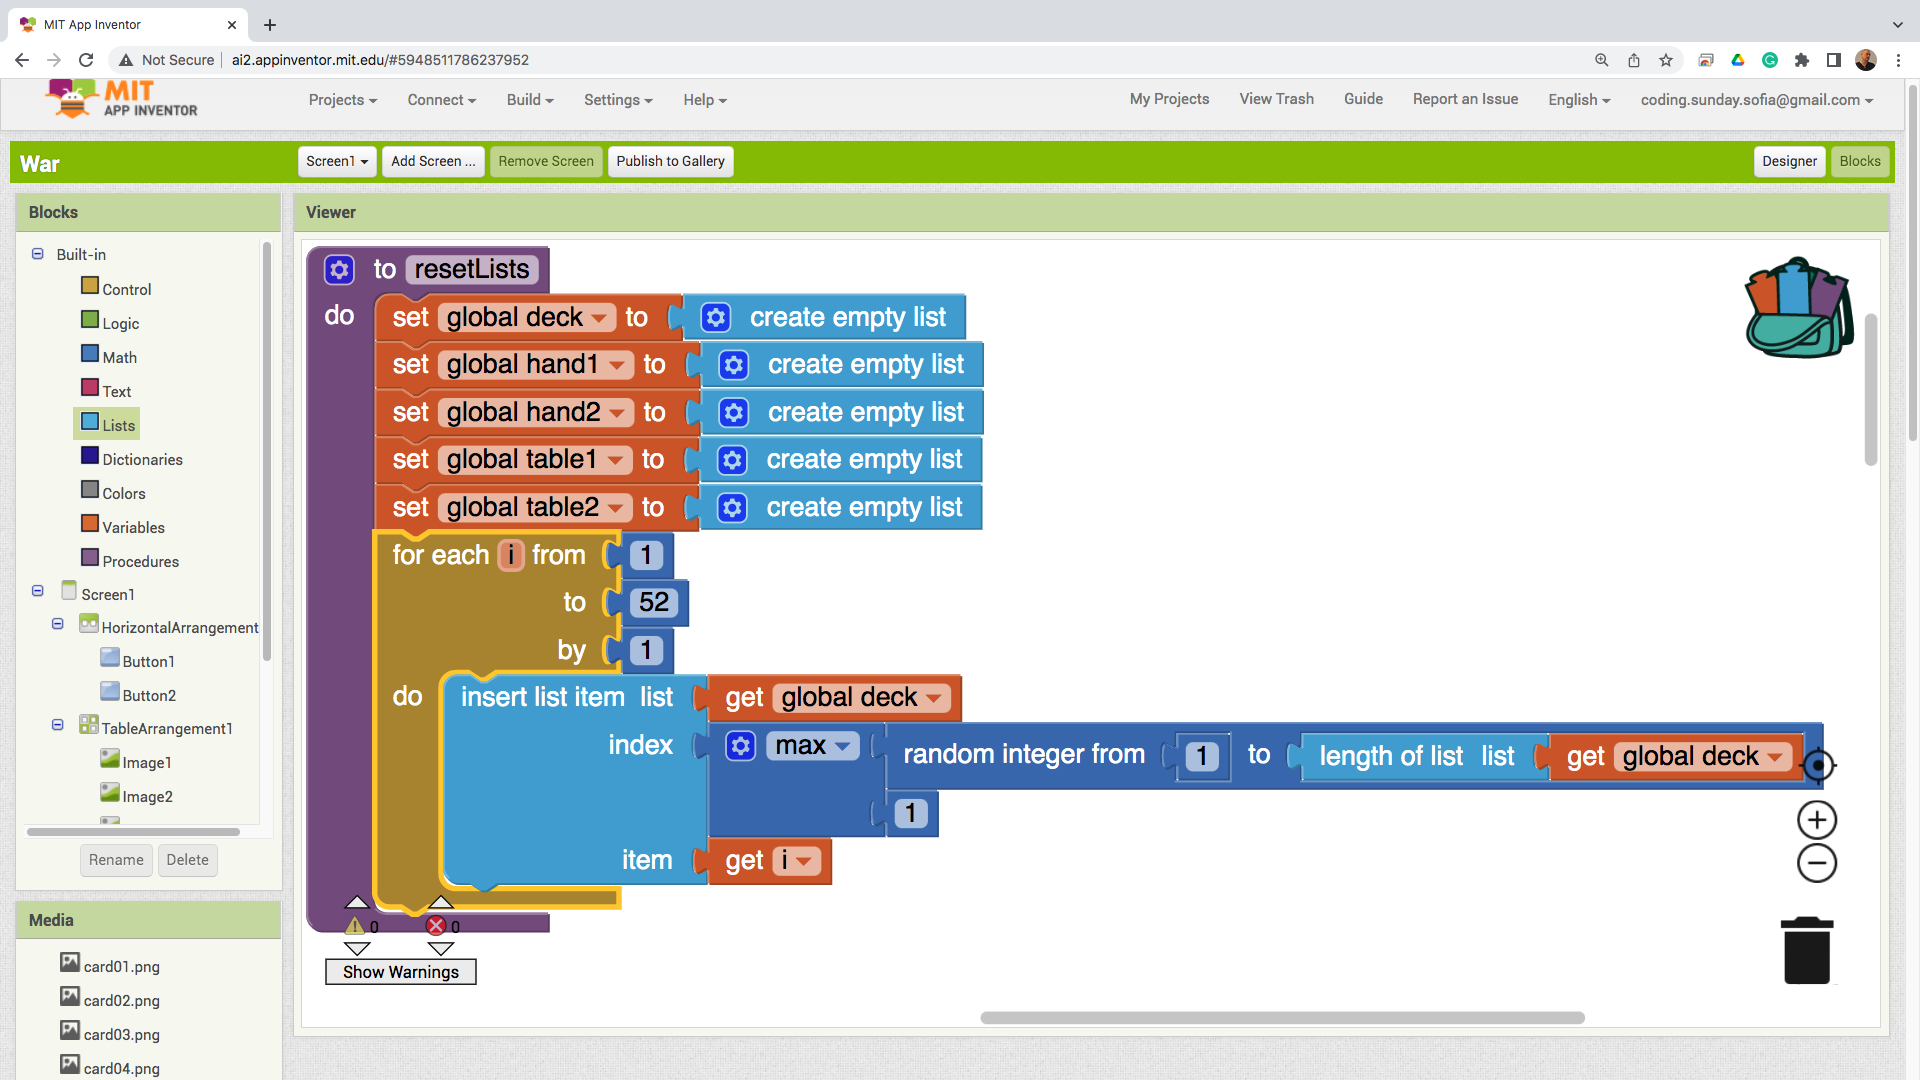
\includegraphics[width=1.0\linewidth,height=0.5\linewidth]{fig100012.png}
   \caption{Deck Initialization Cycle}
\label{fig100012}
\end{figure}

After the main deck is shuffled, the cards are dealt to both players. Each player is dealt half of the cards from the main deck, which are recorded in two auxiliary lists (Fig. \ref{fig100013}). The step in this cycle is 2 because the even cards go to one player, and the odd cards go to the other.

\begin{figure}[H]
   \centering
   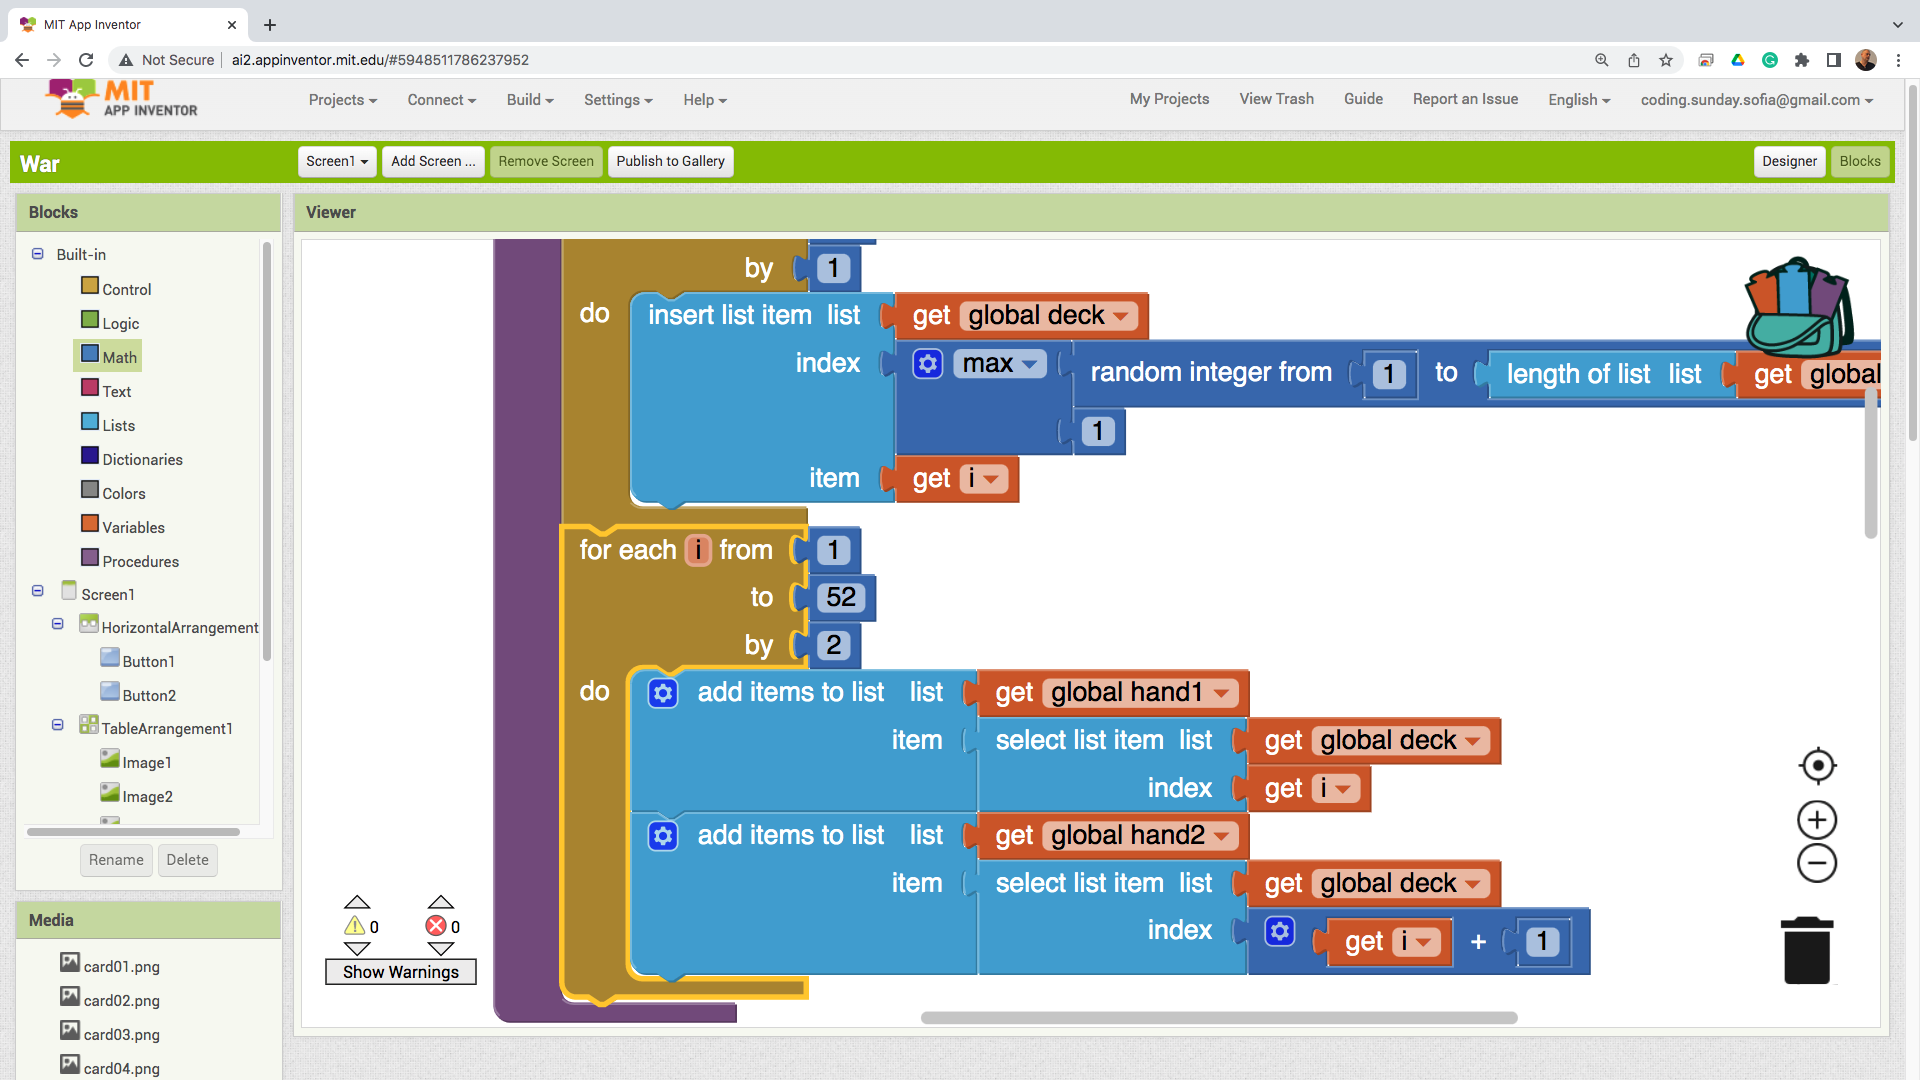
\includegraphics[width=1.0\linewidth,height=0.5\linewidth]{fig100013.png}
   \caption{Dealing the cards}
\label{fig100013}
\end{figure}

After the cards are dealt, the main deck can be assumed to be empty (Fig. \ref{fig100014}).

\begin{figure}[H]
   \centering
   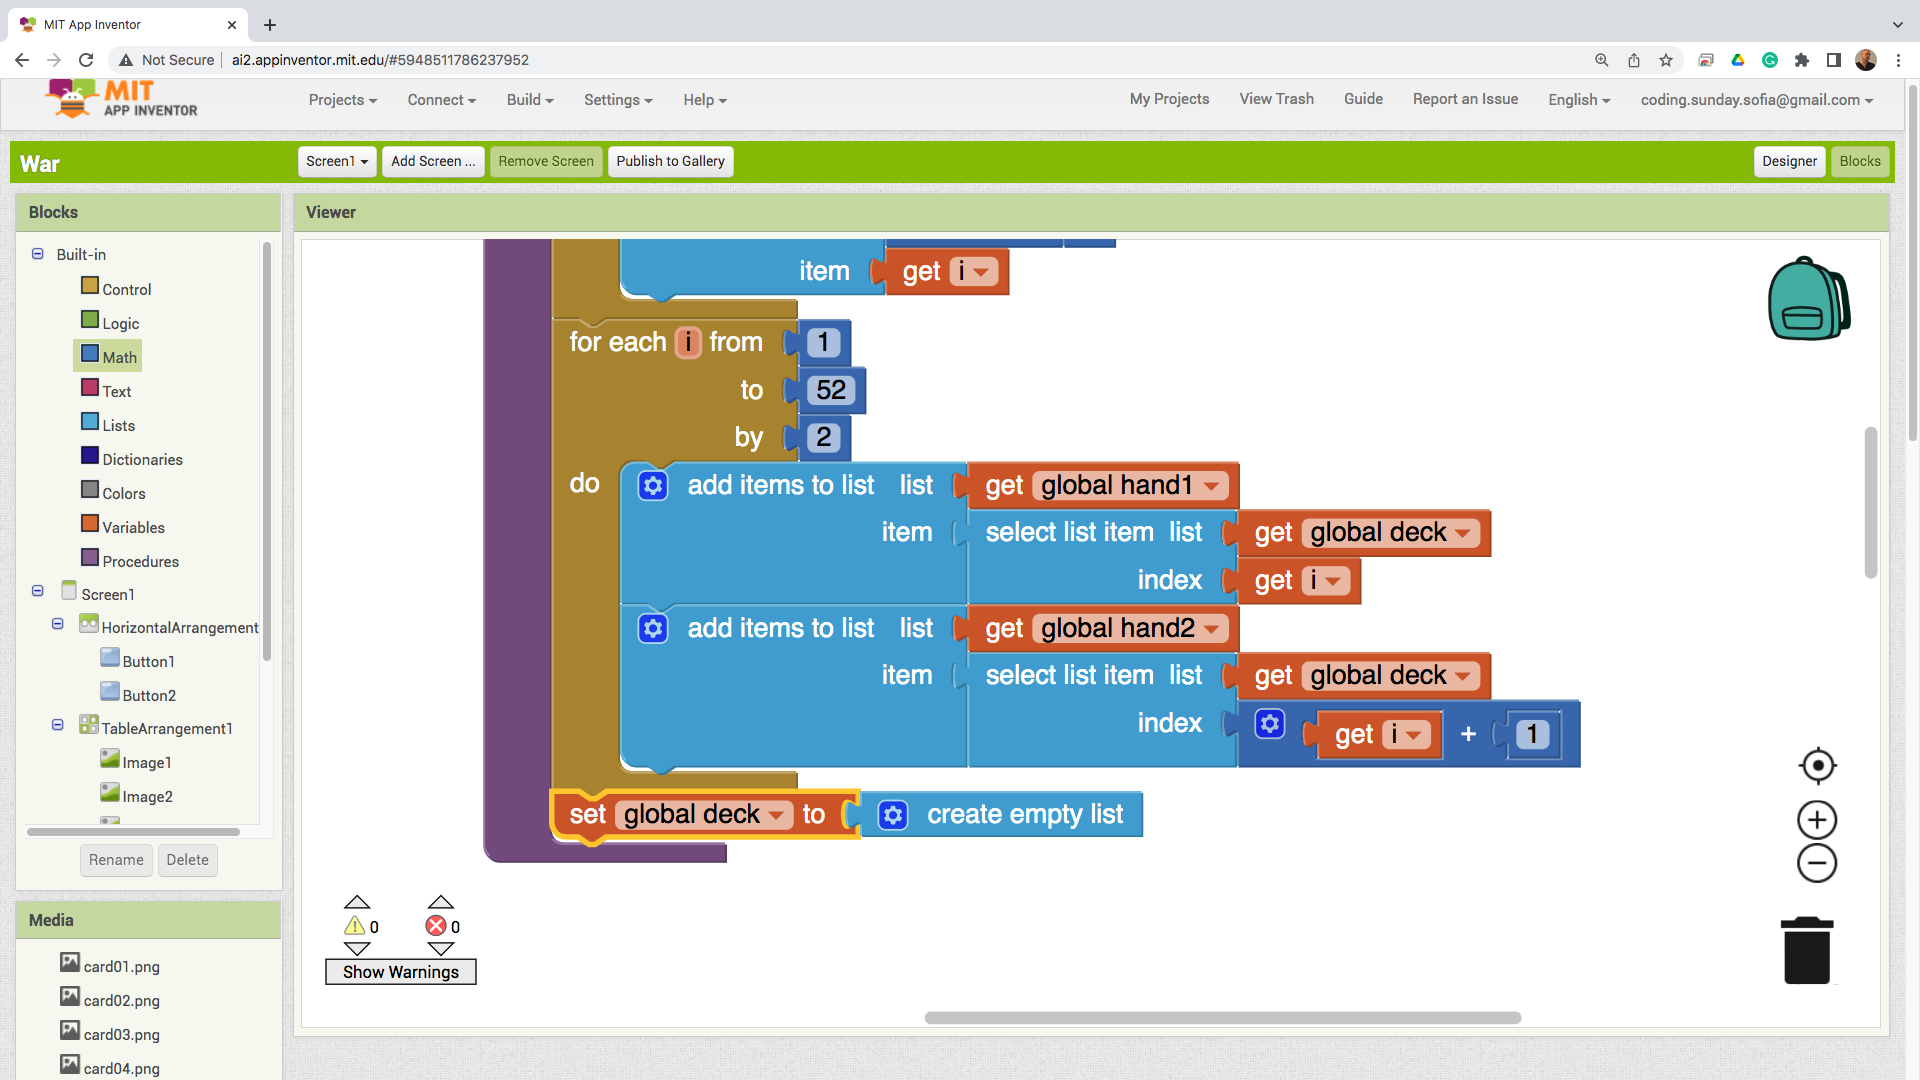
\includegraphics[width=1.0\linewidth,height=0.5\linewidth]{fig100014.png}
   \caption{Reset Deck}
\label{fig100014}
\end{figure}

Internal structures need to be initialized in two situations - when the application is launched and when the user decides to start a new game (Fig. \ref{fig100015}).

\begin{figure}[H]
   \centering
   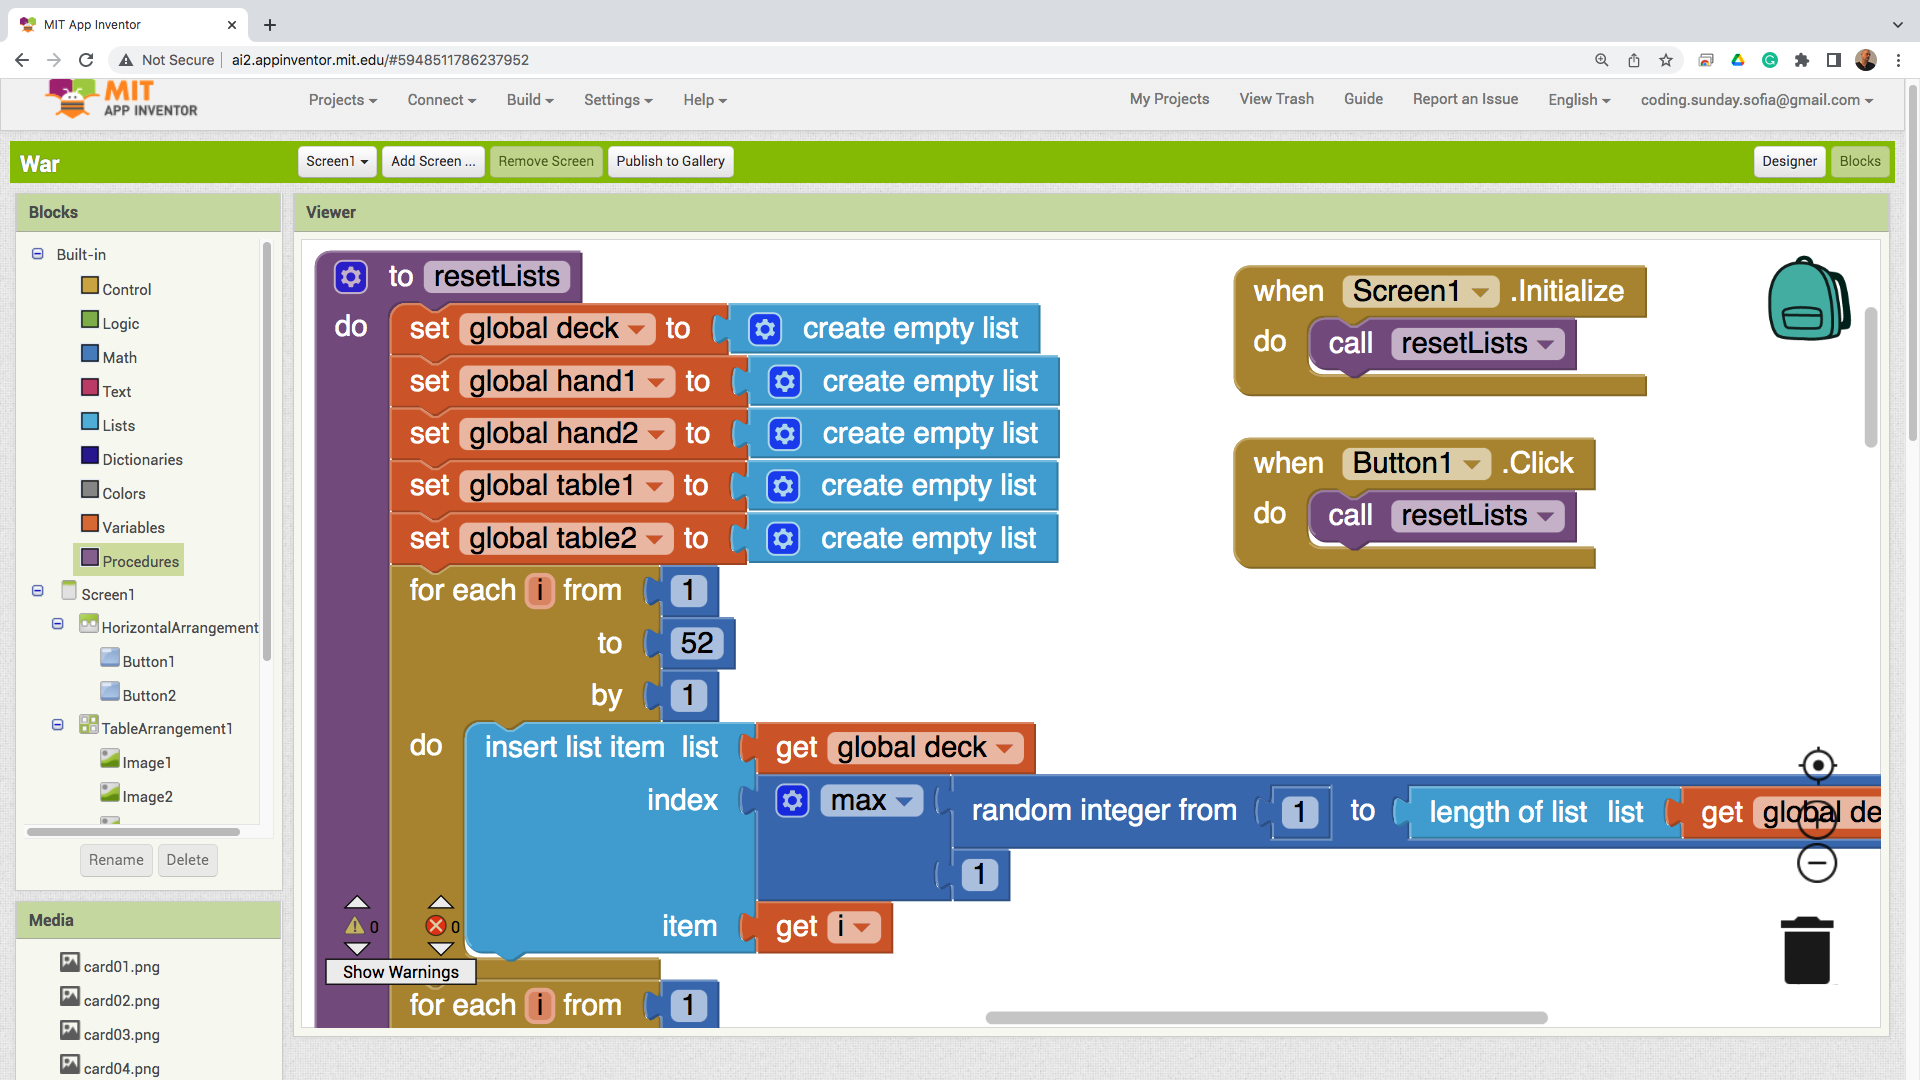
\includegraphics[width=1.0\linewidth,height=0.5\linewidth]{fig100015.png}
   \caption{Initialization Calls}
\label{fig100015}
\end{figure}

The following helper procedure removes images if loaded in the image viewer components (Fig. \ref{fig100016}). This procedure is helpful on any turn when it has already been determined which player will collect the cards from the table.

\begin{figure}[H]
   \centering
   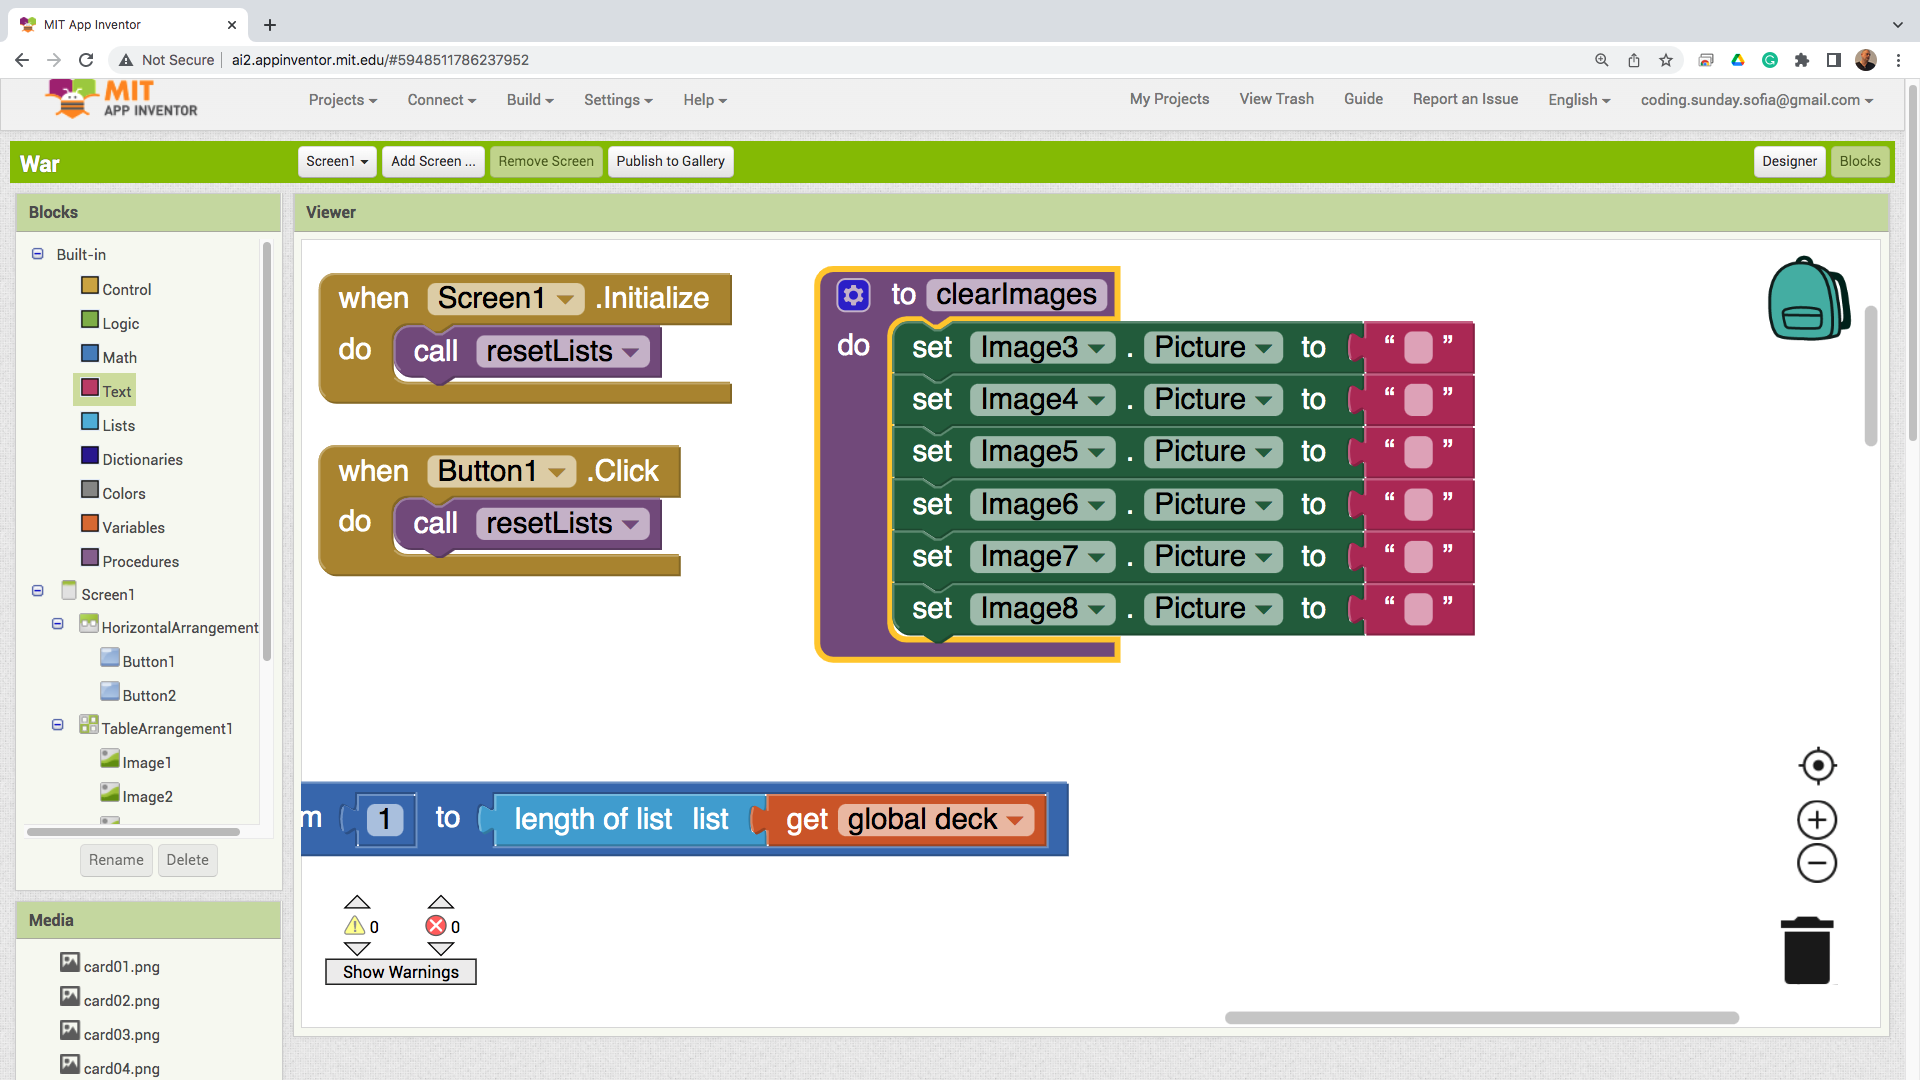
\includegraphics[width=1.0\linewidth,height=0.5\linewidth]{fig100016.png}
   \caption{Image Clearing Procedure}
\label{fig100016}
\end{figure}

Pressing the second button advances the game one step forward. His first task is to clean up the displayed cards from the previous move (Fig. \ref{fig100017}). Then follows a cascade of possible situations.

\begin{figure}[H]
   \centering
   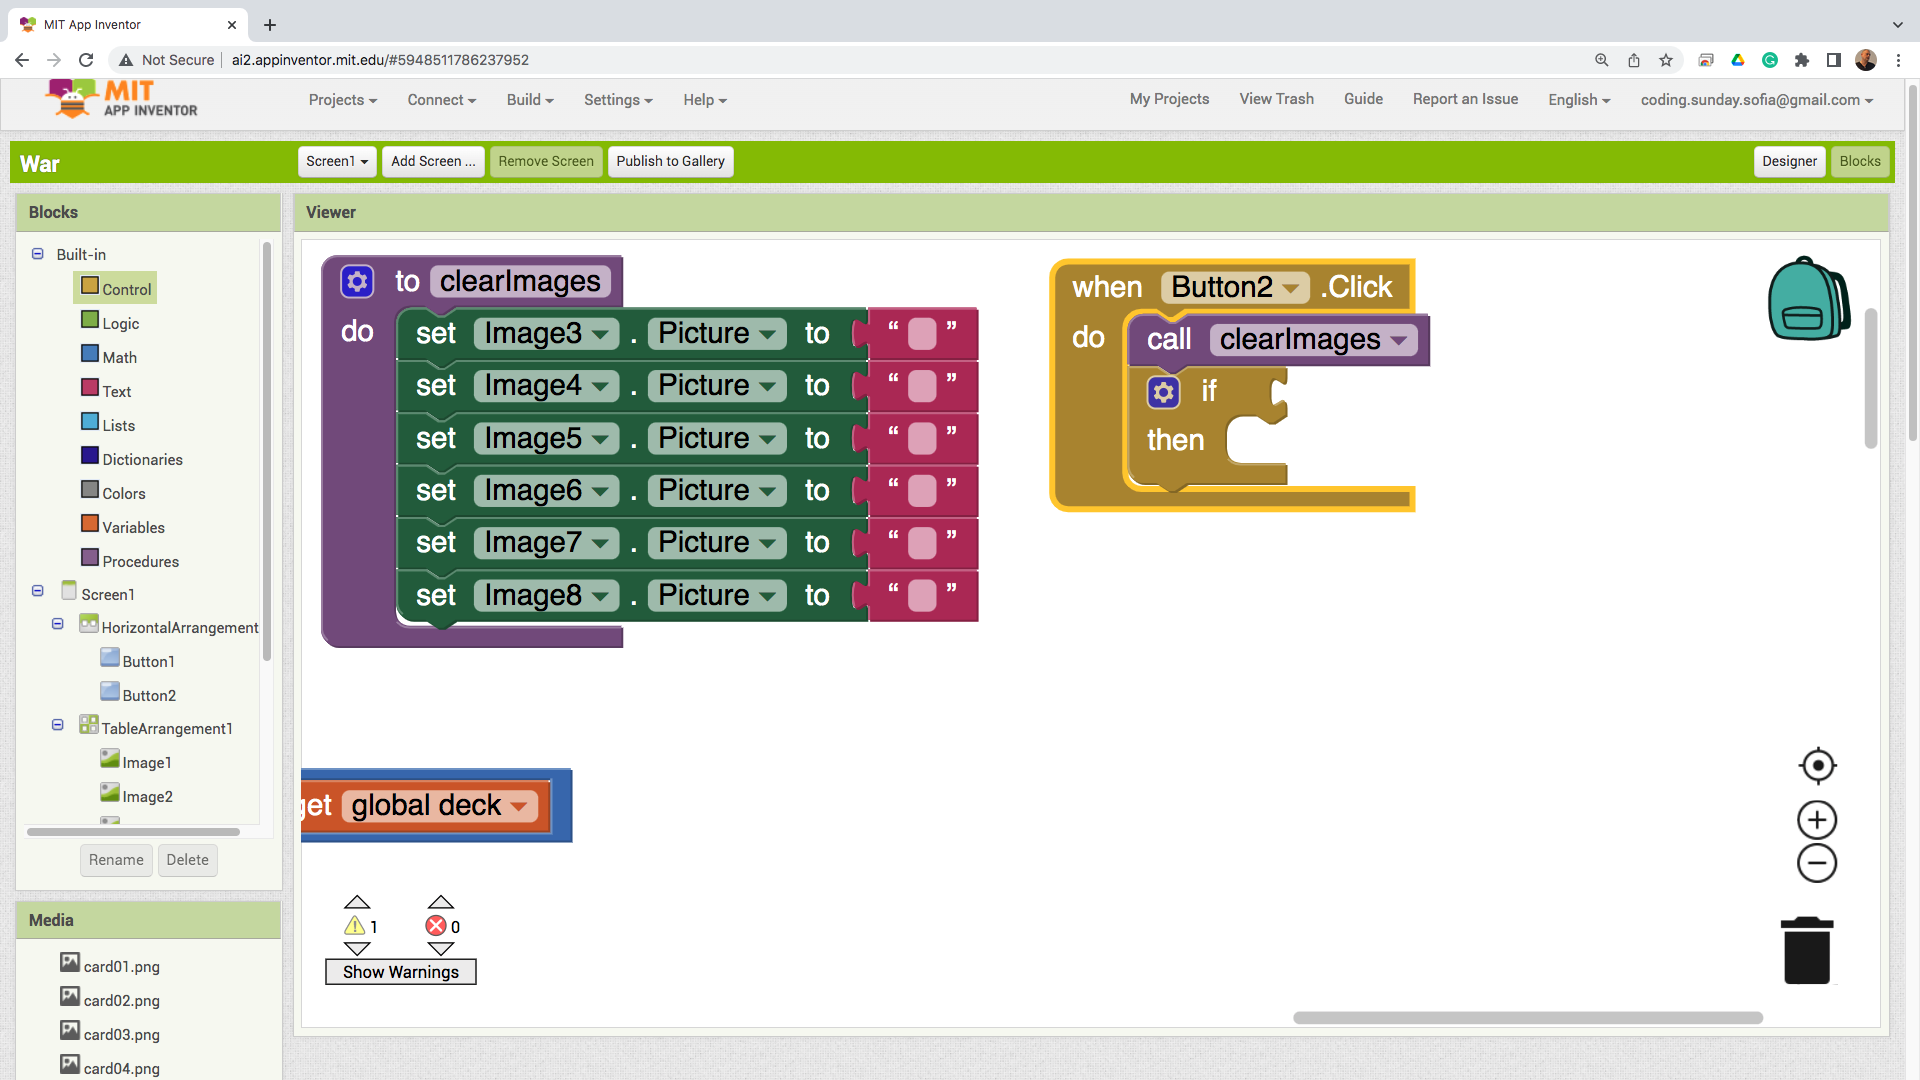
\includegraphics[width=1.0\linewidth,height=0.5\linewidth]{fig100017.png}
   \caption{Catch event for next game step}
\label{fig100017}
\end{figure}

The first two situations on the game board are when one player has cards in his hand, the other does not, and there are no cards on the table (Fig. \ref{fig100018}). In this situation, the player who has cards in his hand is the winner.

\begin{figure}[H]
   \centering
   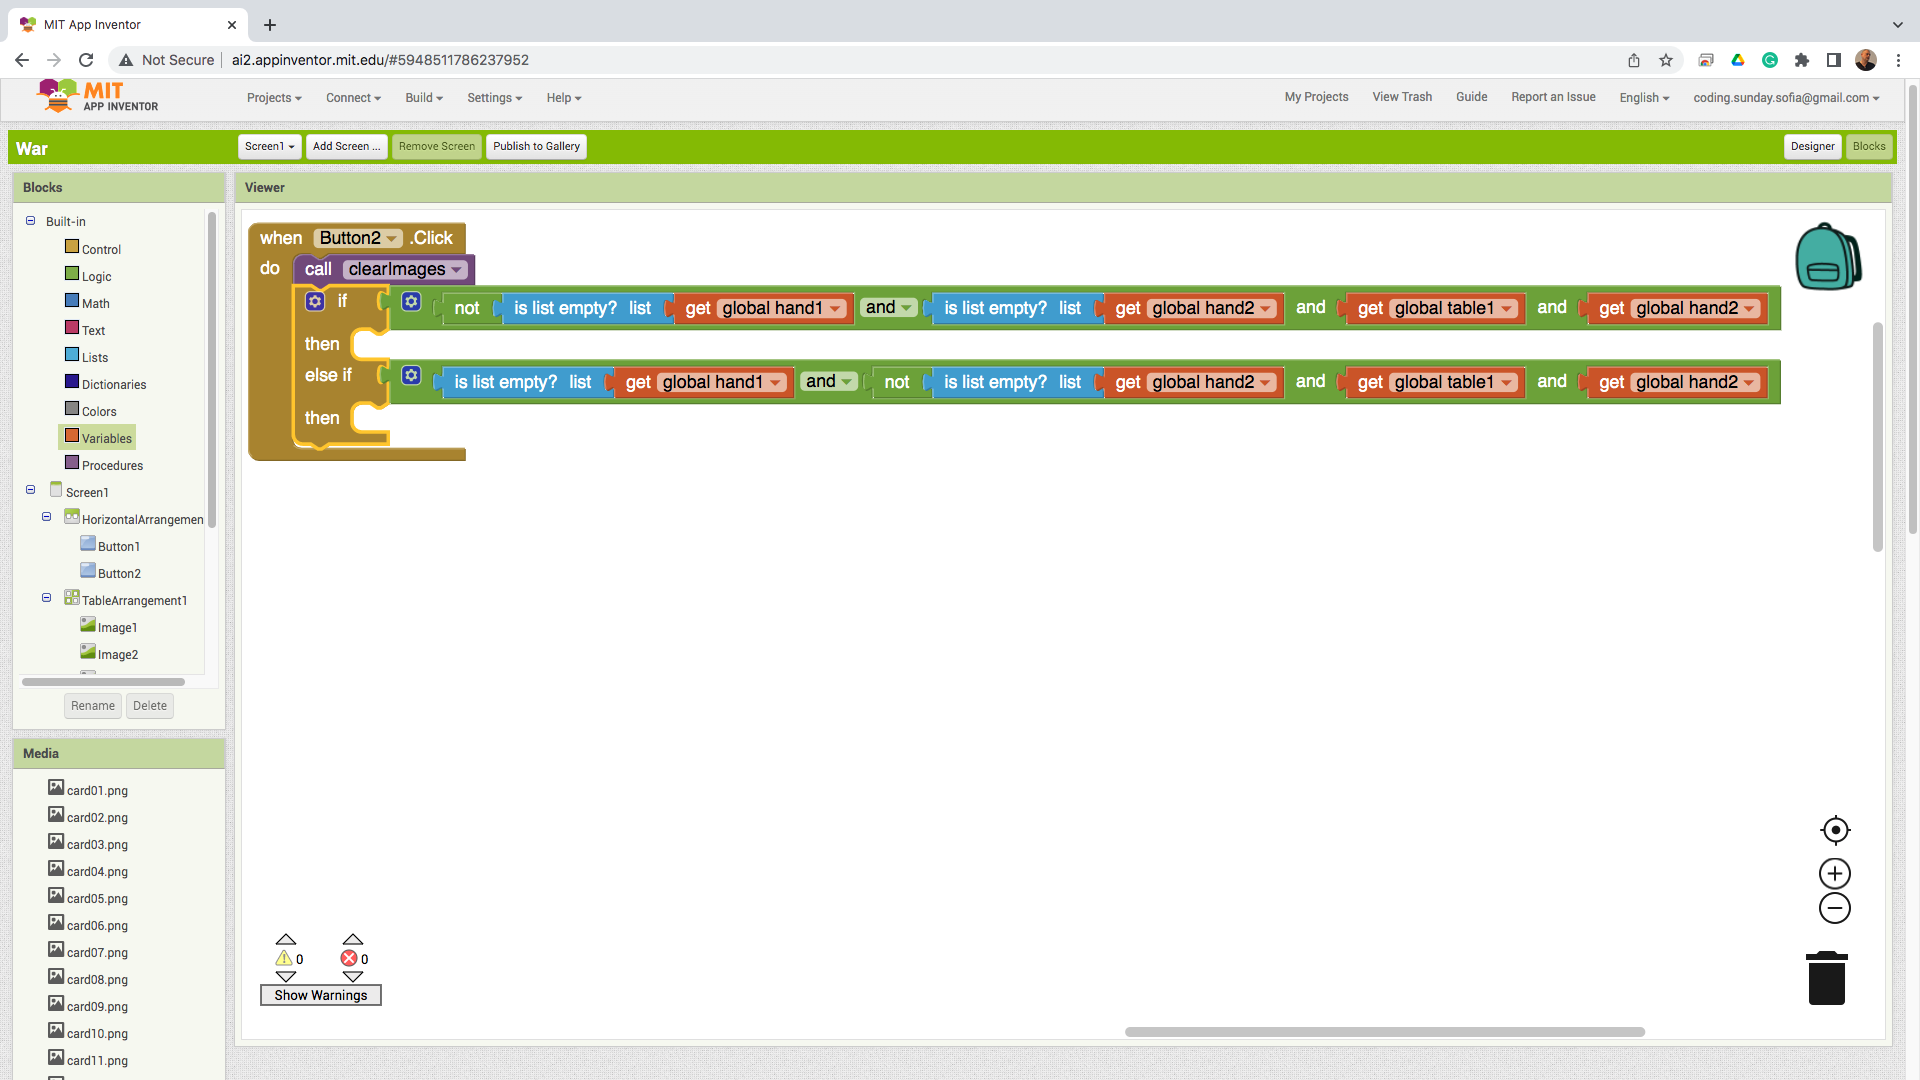
\includegraphics[width=1.0\linewidth,height=0.5\linewidth]{fig100018.png}
   \caption{Situations with already determined winner}
\label{fig100018}
\end{figure}

The second two situations (Fig. \ref{fig100019}) are when there are no cards on the table, that is, they must be drawn from the decks, and when there are cards on the table, and it is necessary to determine which player wins the round.

\begin{figure}[H]
   \centering
   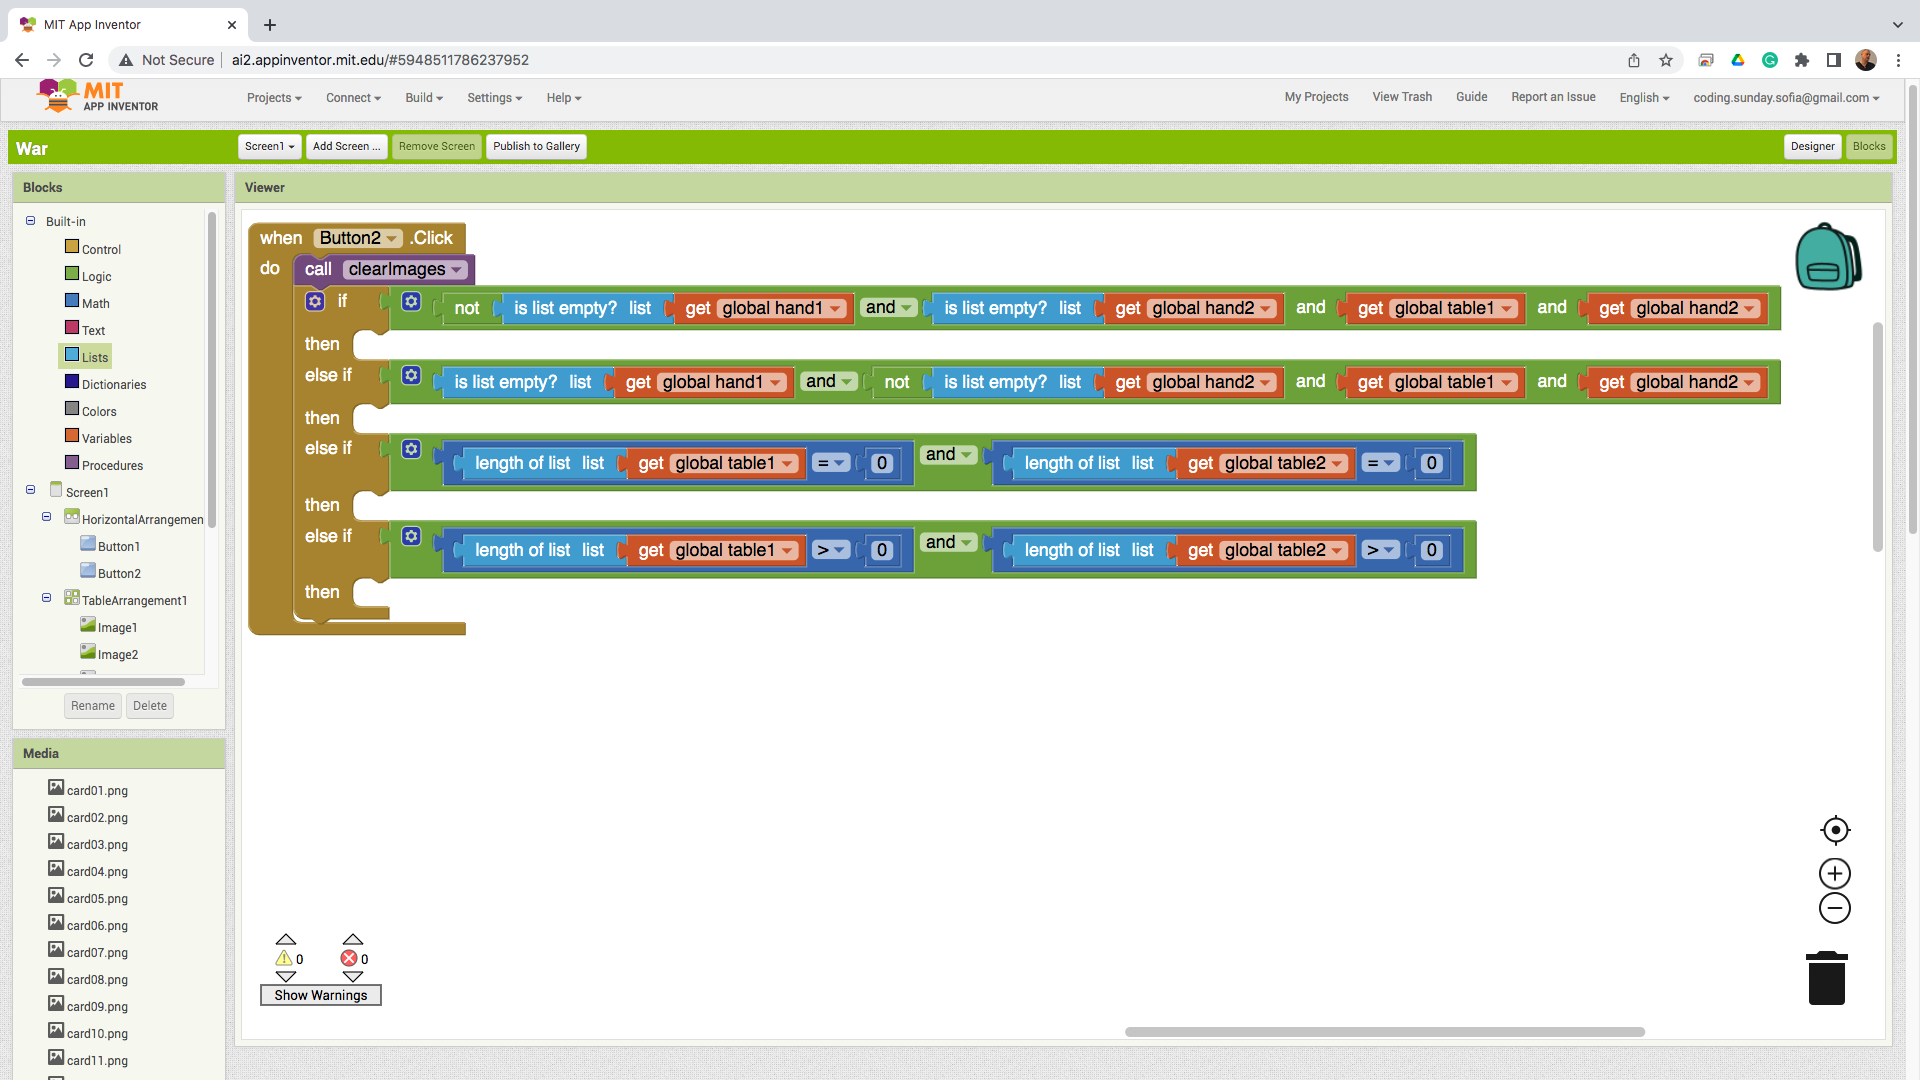
\includegraphics[width=1.0\linewidth,height=0.5\linewidth]{fig100019.png}
   \caption{Situations according to the presence of cards on the table}
\label{fig100019}
\end{figure}

Only the winner is announced in a message for the first two conditions. Auxiliary functions are defined for the second two states. Immediately after the possible states follows an auxiliary function for updating the visual space (Fig. \ref{fig100020}).

\begin{figure}[H]
   \centering
   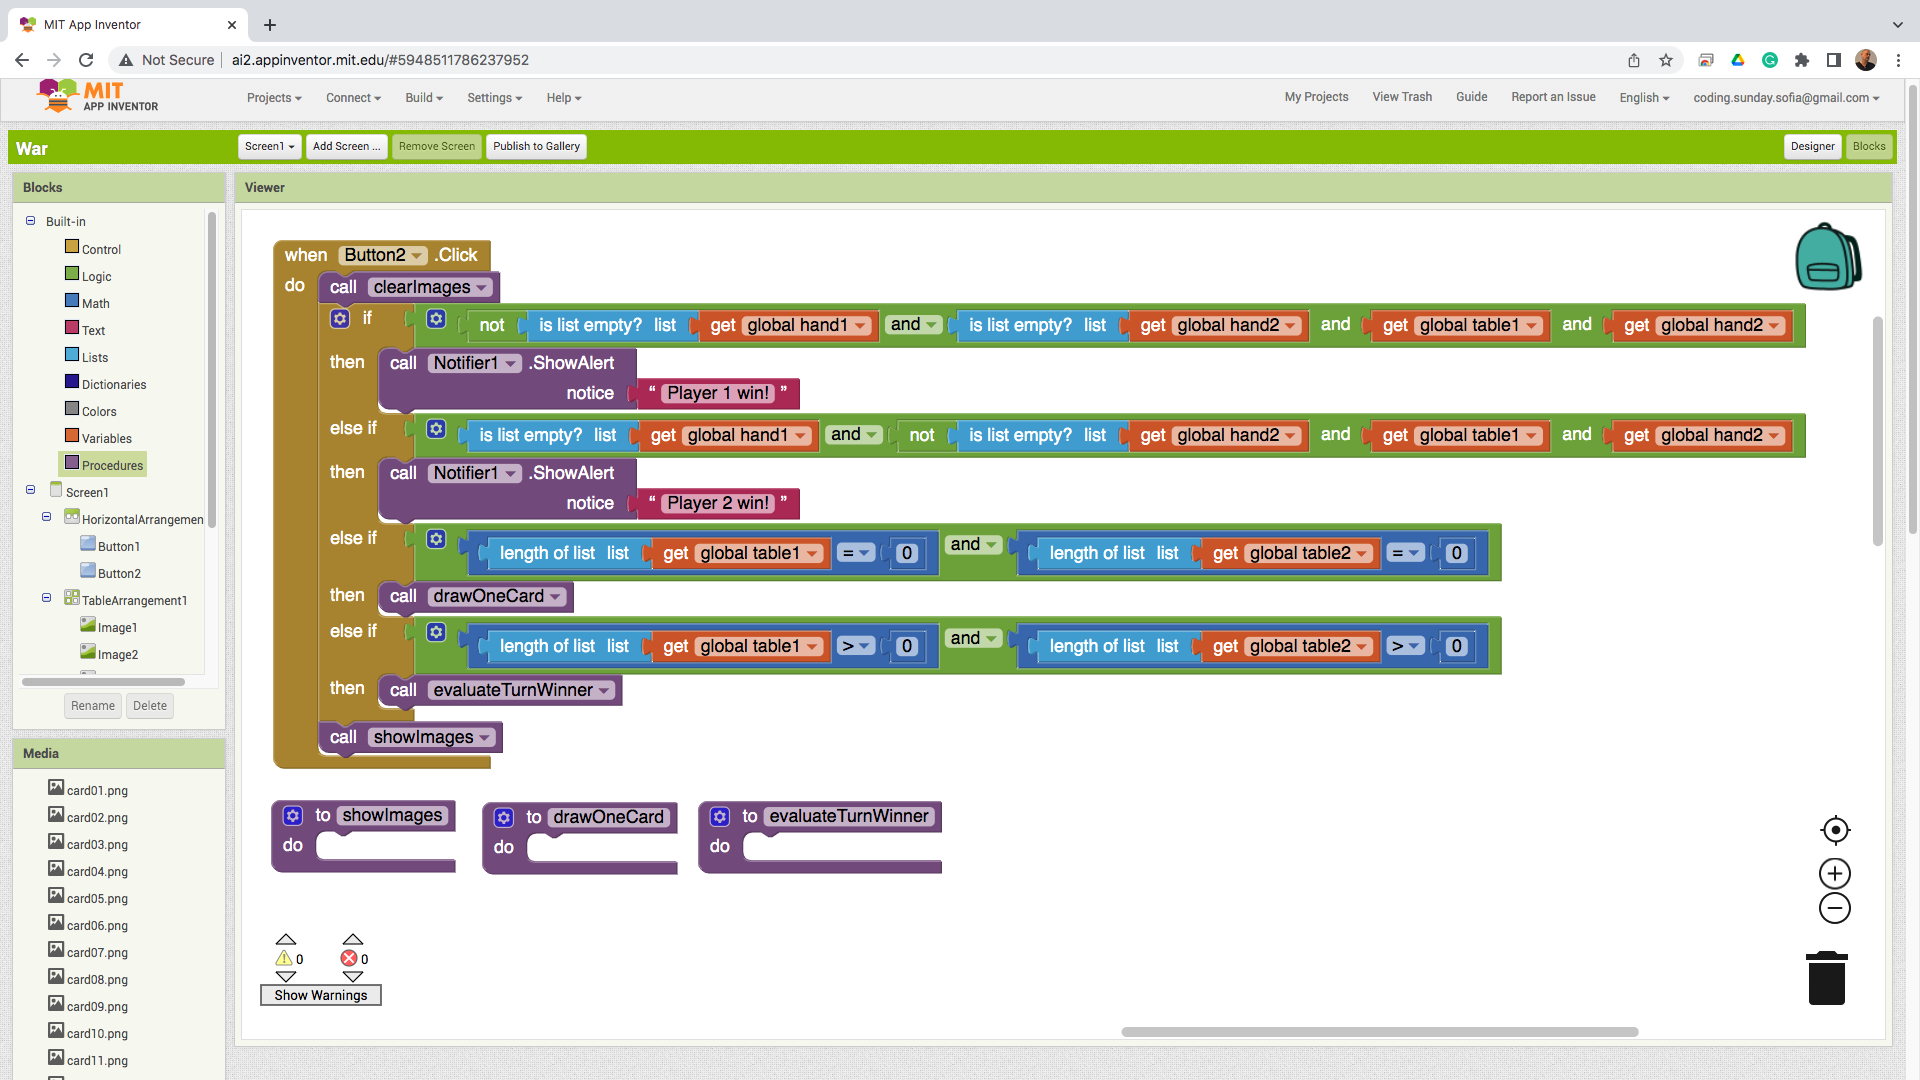
\includegraphics[width=1.0\linewidth,height=0.5\linewidth]{fig100020.png}
   \caption{Helper functions to work out different situations}
\label{fig100020}
\end{figure}

In the most complex case, the auxiliary function for visualizing the cards on the table shows up to three cards per player, a total of six. When there is no state of war, one card is visualized. When there is a state of war, the three cards of the last war are visualized (wars may be several in a row). Visualization occurs in two consecutive cycles (Fig. \ref{fig100021}).

\begin{figure}[H]
   \centering
   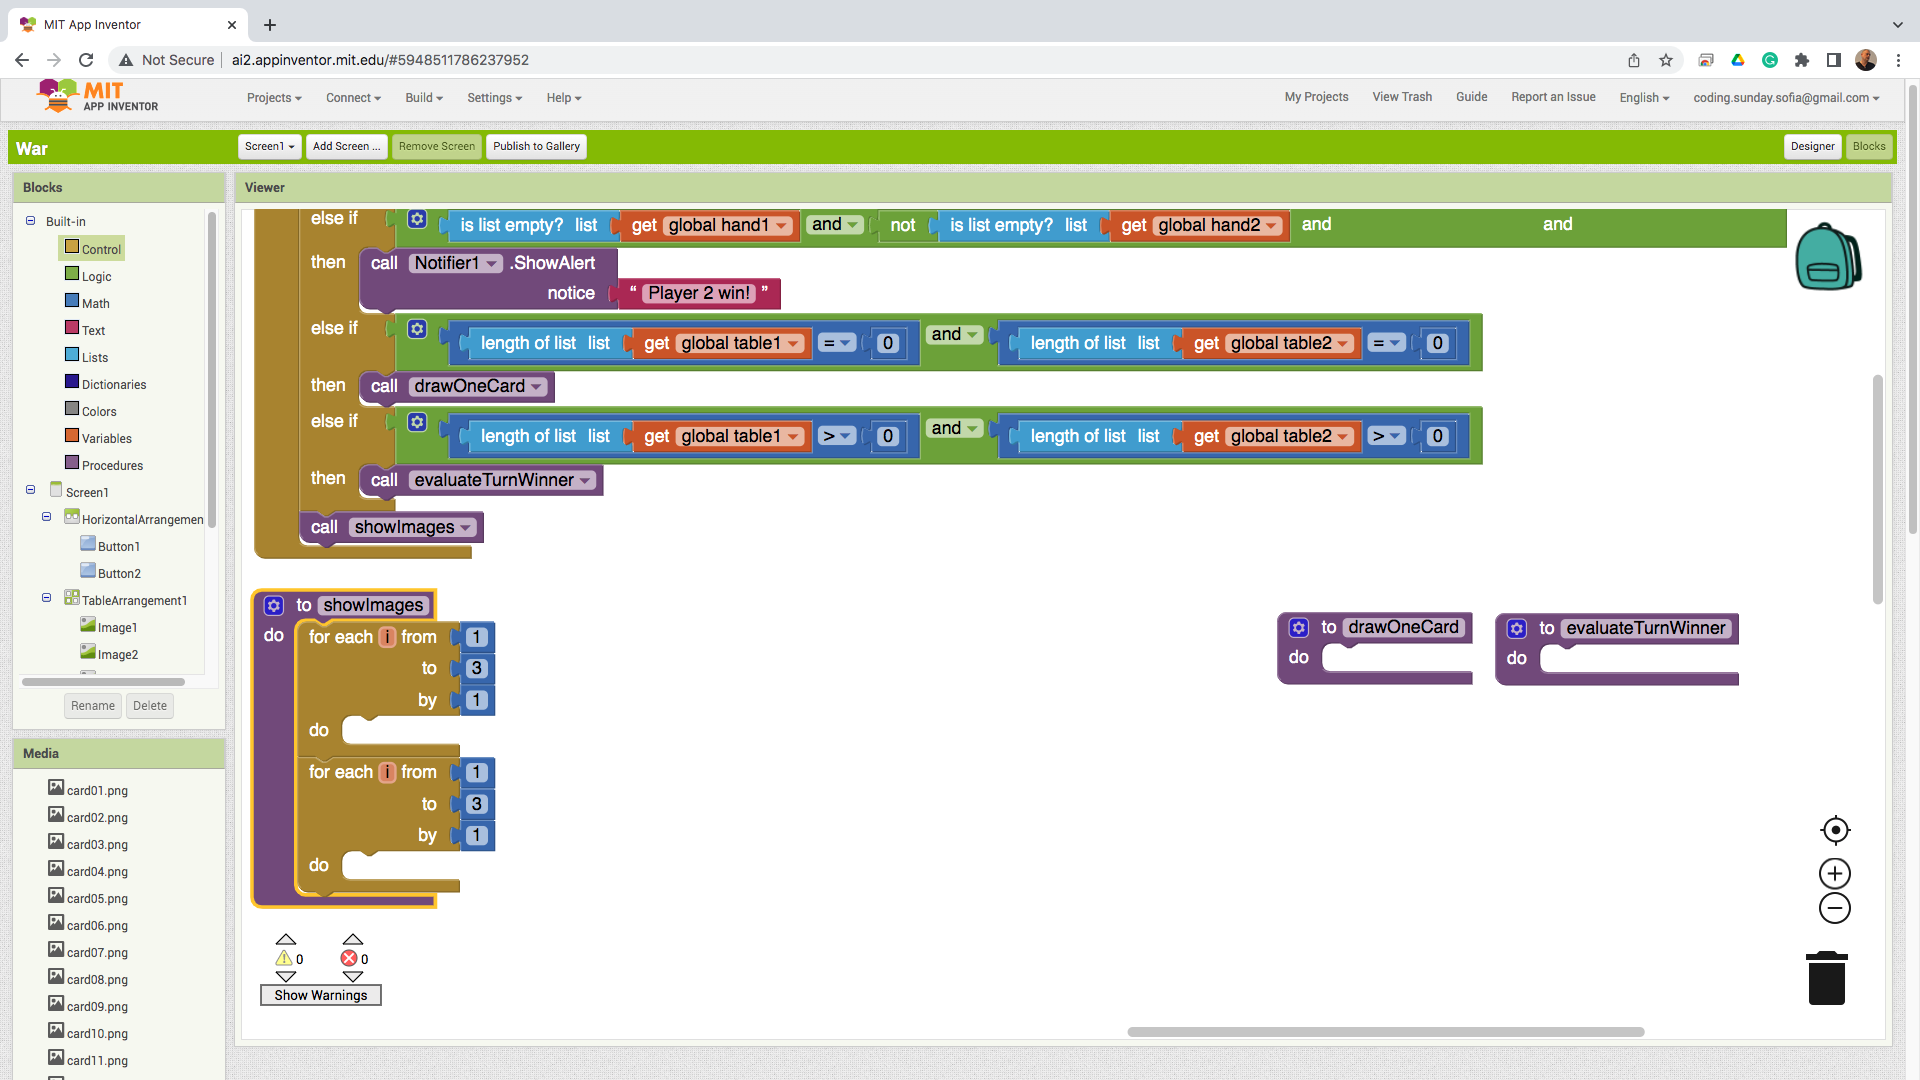
\includegraphics[width=1.0\linewidth,height=0.5\linewidth]{fig100021.png}
   \caption{Cycles to view cards on the table}
\label{fig100021}
\end{figure}

If there are not enough items in the card lists on the table, then the rendering loop must be aborted (Fig. \ref{fig100022}). An example is when a state of war appears, but one player only has two last cards left.

\begin{figure}[H]
   \centering
   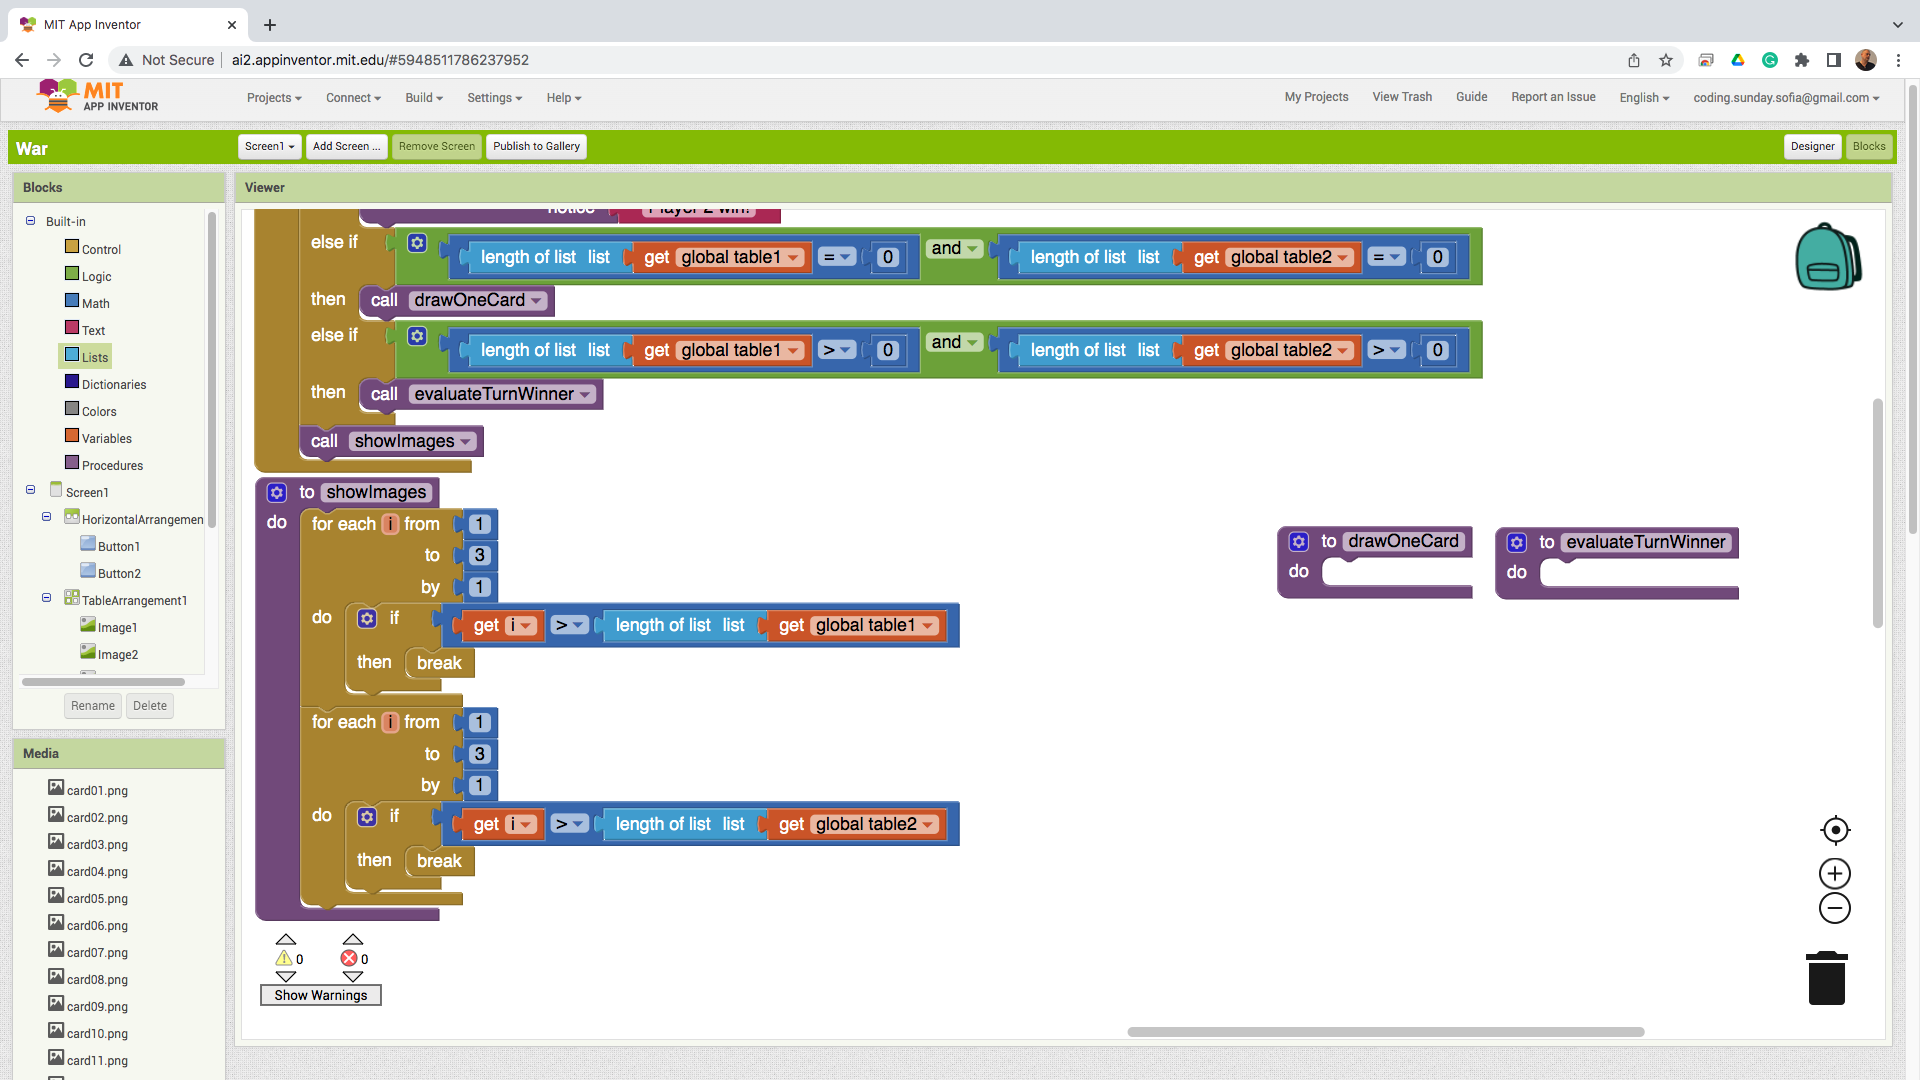
\includegraphics[width=1.0\linewidth,height=0.5\linewidth]{fig100022.png}
   \caption{Stop preview when cards are missing}
\label{fig100022}
\end{figure}

If there are enough cards on the table, the image viewer component displays that image from the list of images, which is specified as an index in the list of cards on the table (Fig. \ref{fig100023}).

\begin{figure}[H]
   \centering
   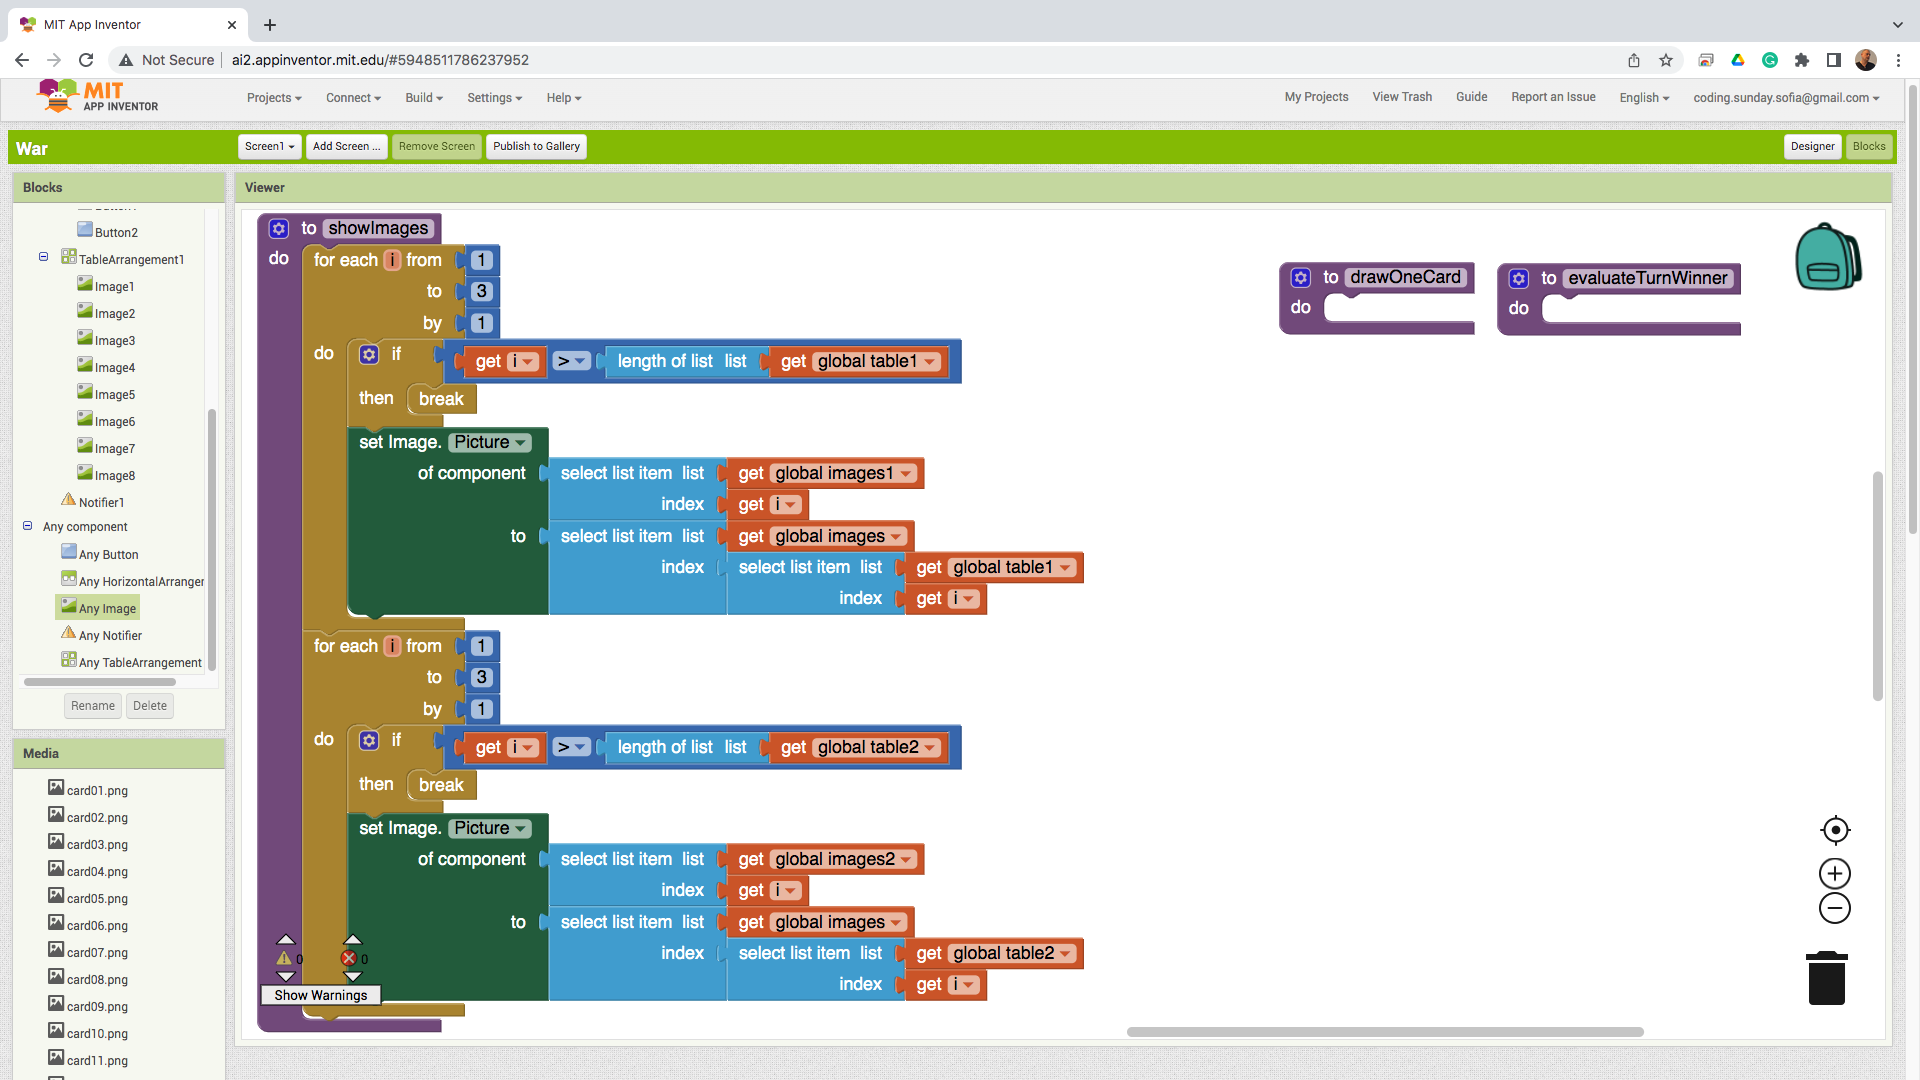
\includegraphics[width=1.0\linewidth,height=0.5\linewidth]{fig100023.png}
   \caption{Determining which images to display}
\label{fig100023}
\end{figure}

To draw a card, each player must take it from their hand first and place it in the card row on the table (Fig. \ref{fig100024}). A card enters the table list and leaves the hand list.

\begin{figure}[H]
   \centering
   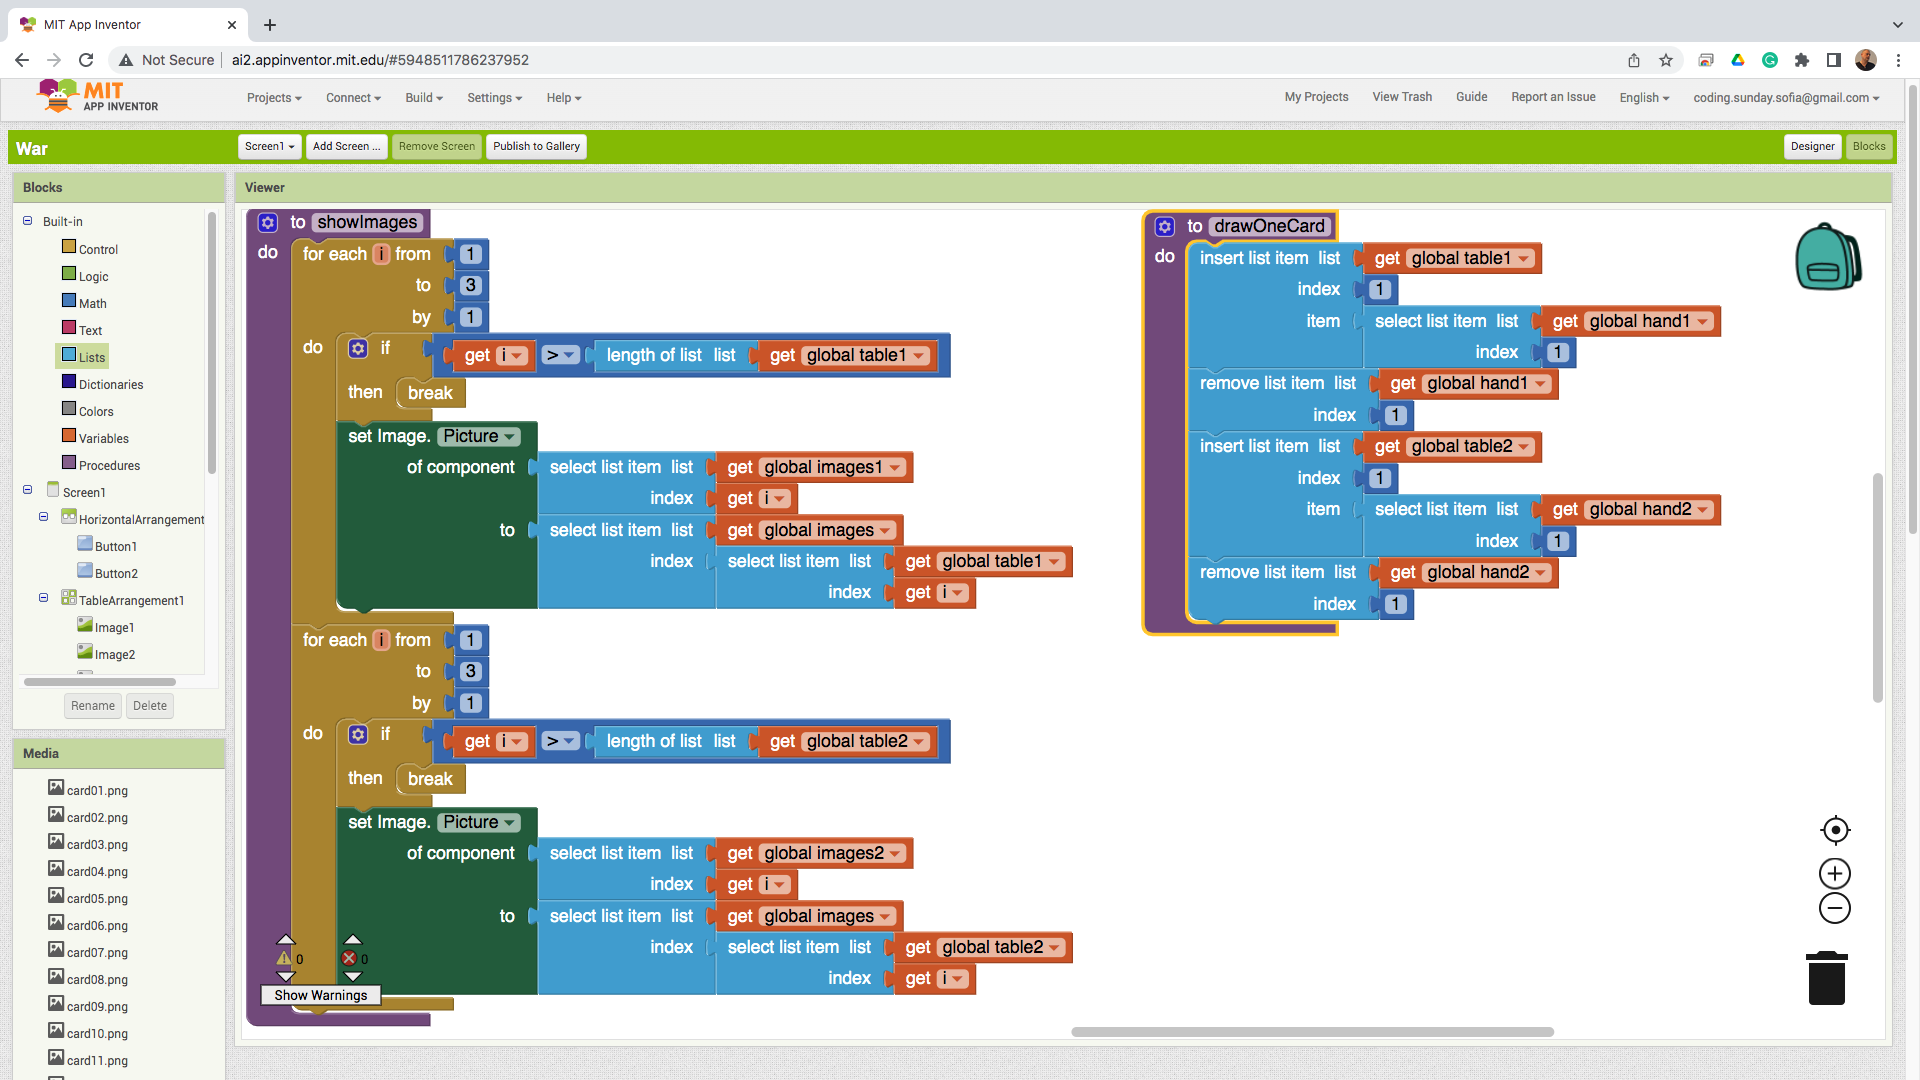
\includegraphics[width=1.0\linewidth,height=0.5\linewidth]{fig100024.png}
   \caption{Download one card at a time}
\label{fig100024}
\end{figure}

When there are cards on the table, three situations are possible - the move is won by the first player, the move is won by the second player, and the players are tied, resulting in a state of war (Fig. \ref{fig100025}). The cards in the main deck are arranged to form four subgroups according to their strength. For this reason, it is easy to determine which card wins in an integer division over two. One must be subtracted because the numbering in the main deck starts from one and goes up to 52, and integer division can be applied to enumeration from 0 to 51.

\begin{figure}[H]
   \centering
   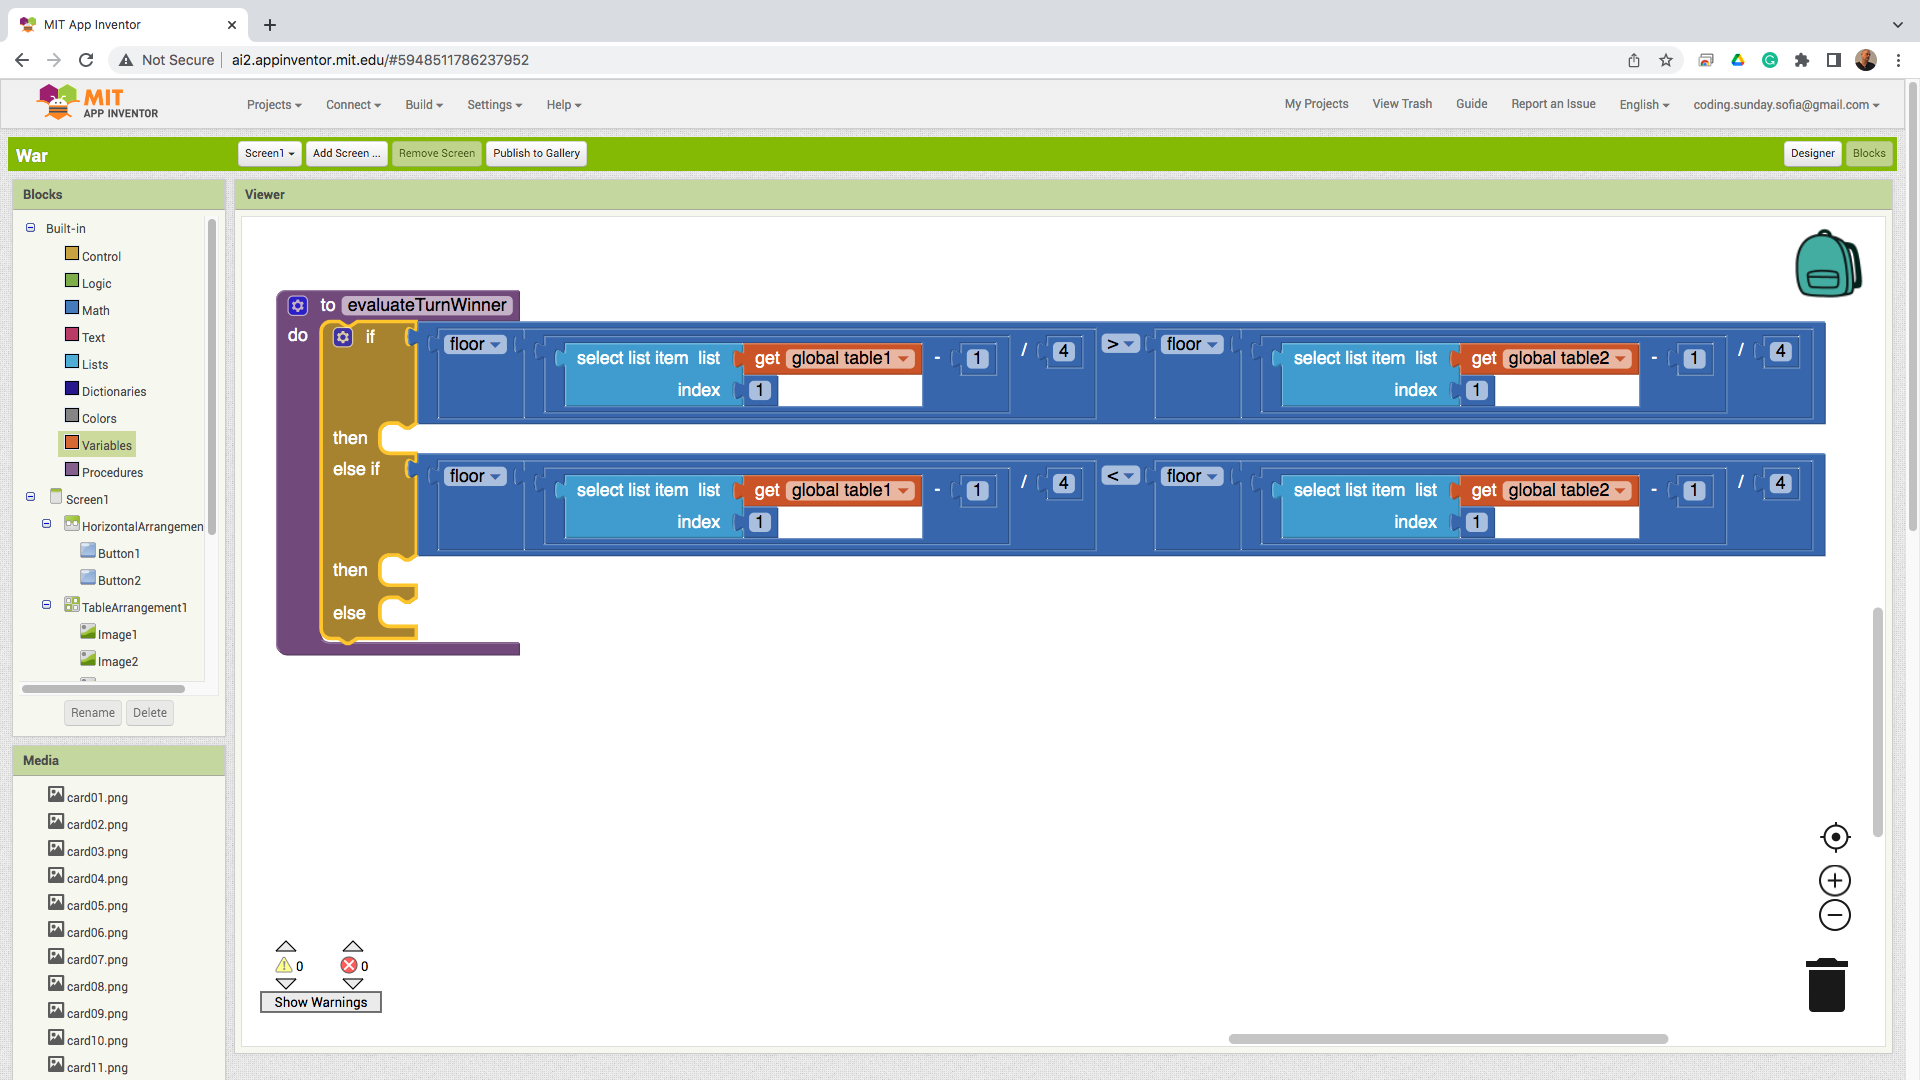
\includegraphics[width=1.0\linewidth,height=0.5\linewidth]{fig100025.png}
   \caption{Possible situations with cards on the table}
\label{fig100025}
\end{figure}

If the first player wins on the current turn, he draws his cards from the table and the cards from the second player's table into his hand. If the second player wins in the current turn, he takes his and his opponent's cards from the table. These actions are performed by filling a list by hand and emptying the lists for the table (Fig. \ref{fig100026}).

\begin{figure}[H]
   \centering
   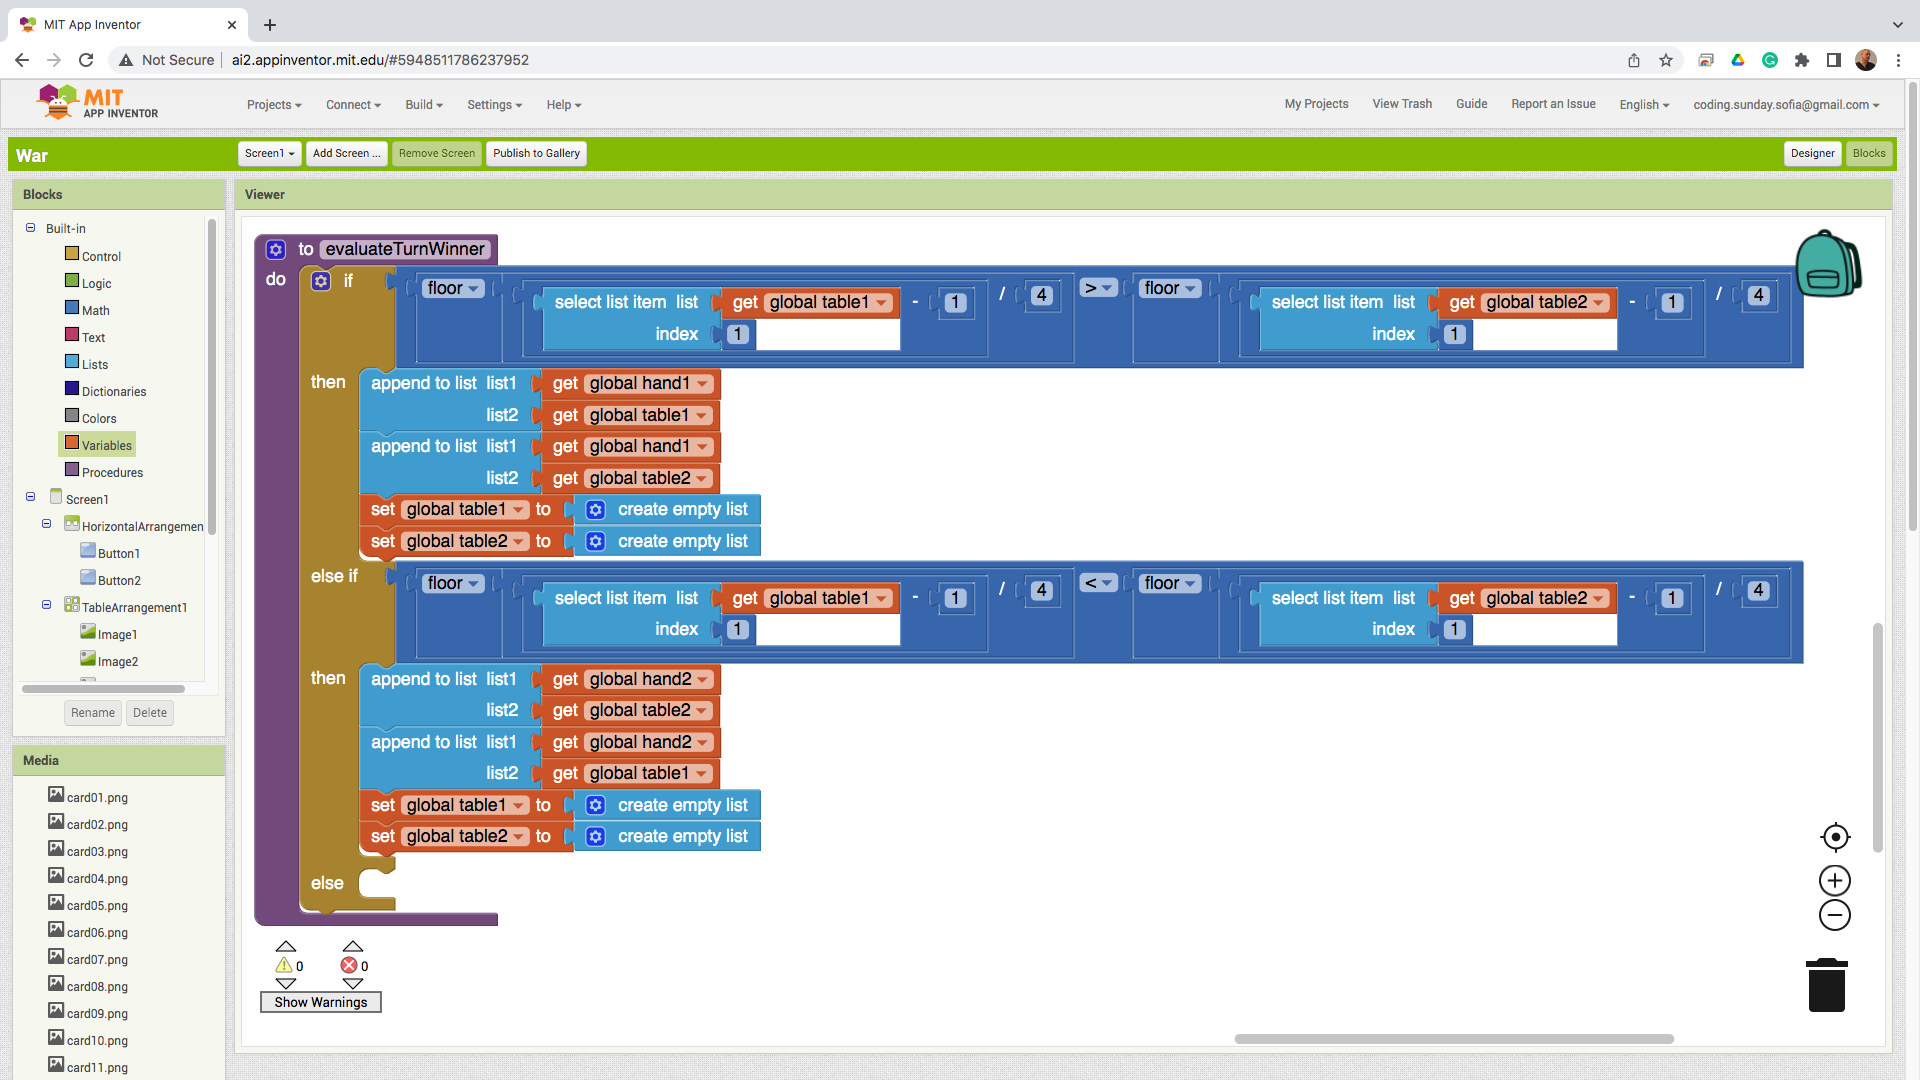
\includegraphics[width=1.0\linewidth,height=0.5\linewidth]{fig100026.png}
   \caption{Collecting the cards after winning a separate turn of the game}
\label{fig100026}
\end{figure}

In a state of war, each player draws three cards to participate in the war. This action occurs in a loop rotating three times (Fig. \ref{fig100027}).

\begin{figure}[H]
   \centering
   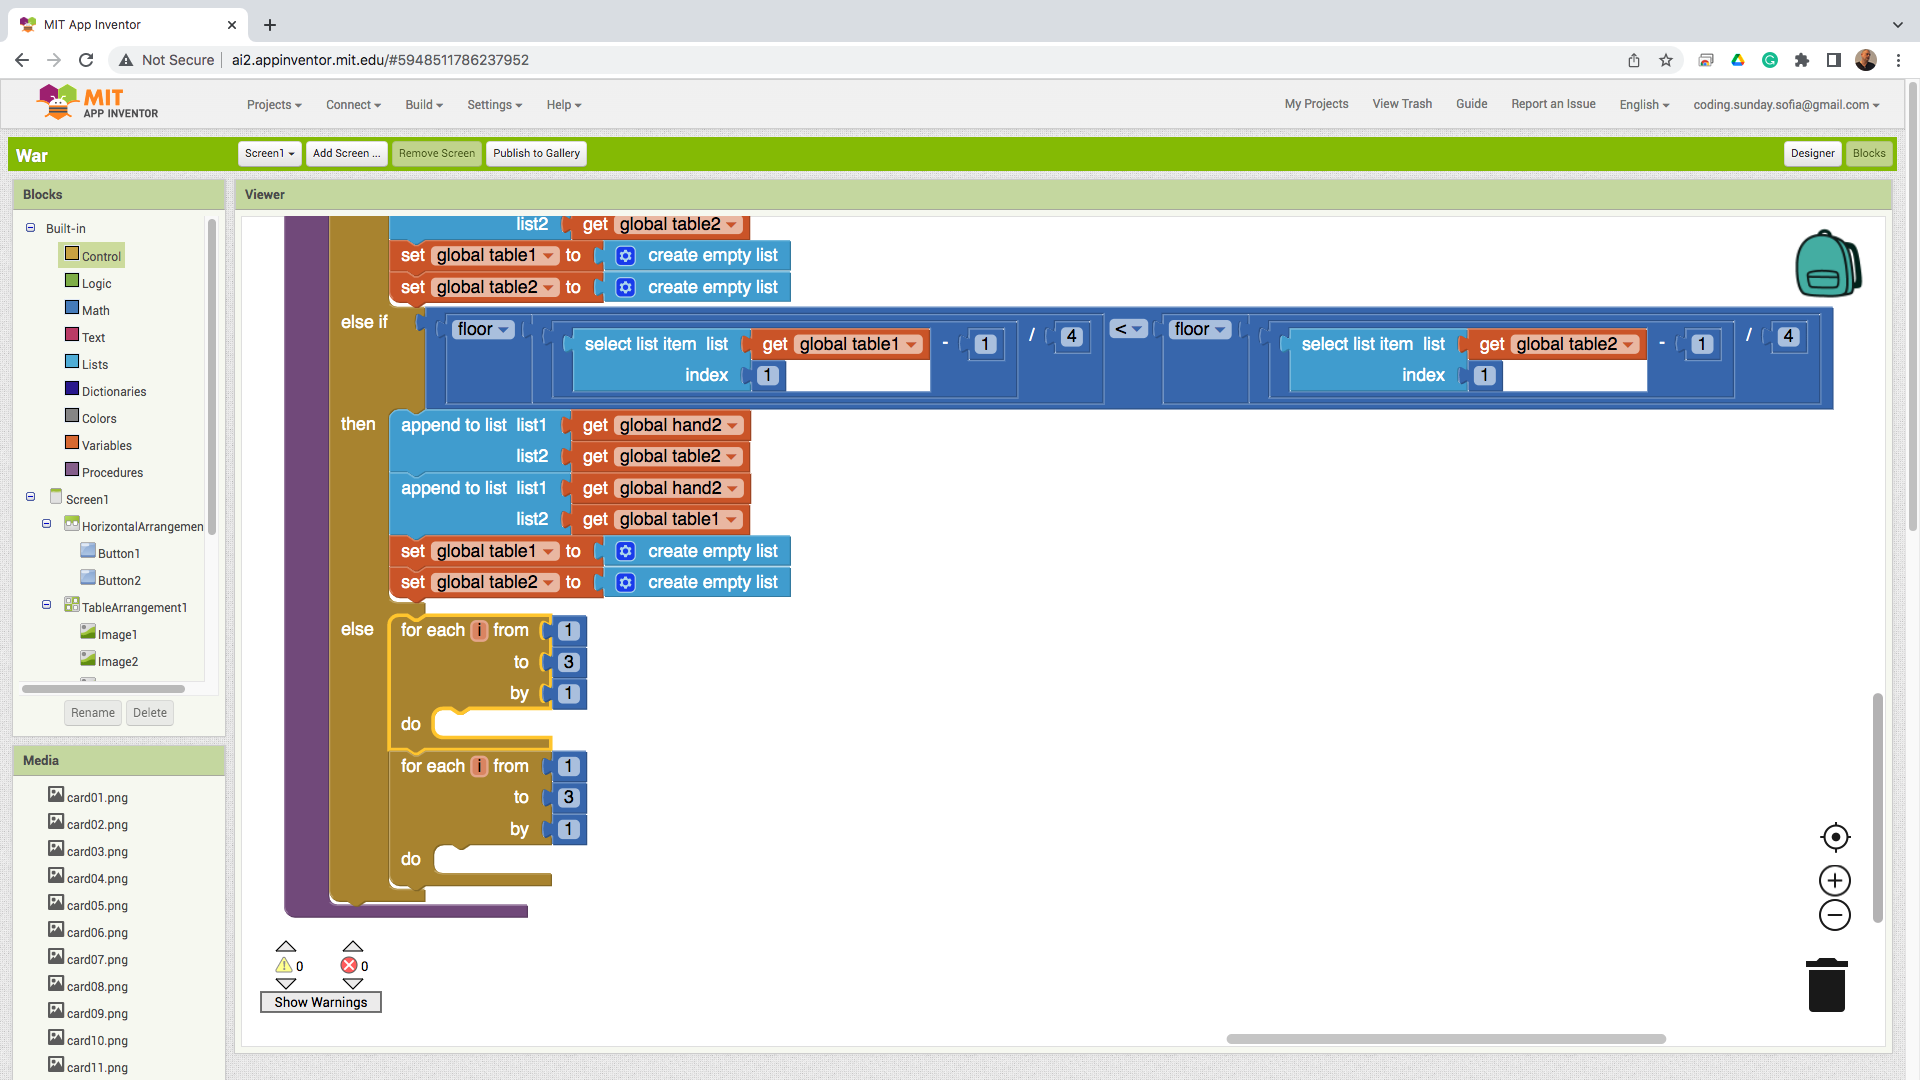
\includegraphics[width=1.0\linewidth,height=0.5\linewidth]{fig100027.png}
   \caption{War map display cycle}
\label{fig100027}
\end{figure}

In the process of drawing cards for the war, it is possible that one of the players runs out of cards and cannot draw, then the draw cycle must be stopped (Fig. \ref{fig100028}).

\begin{figure}[H]
   \centering
   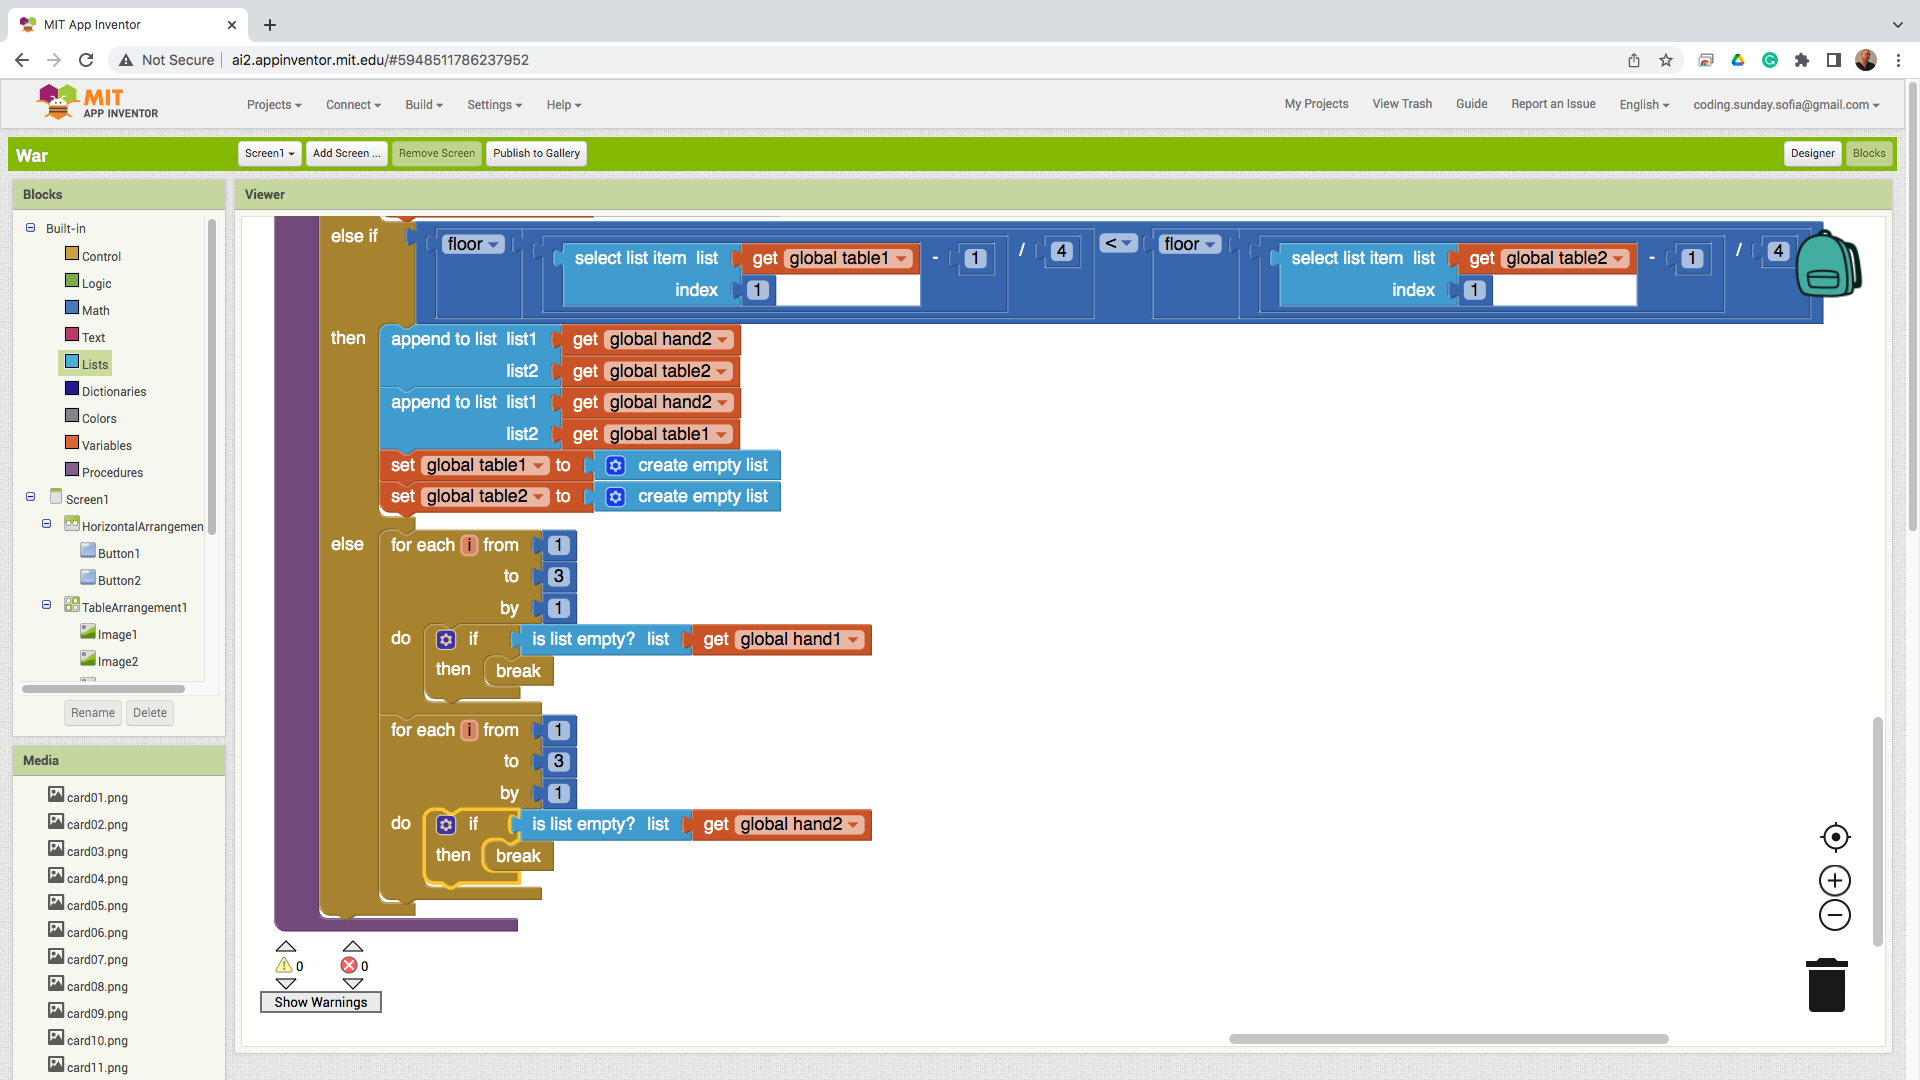
\includegraphics[width=1.0\linewidth,height=0.5\linewidth]{fig100028.png}
   \caption{Stop withdrawal when cards run out}
\label{fig100028}
\end{figure}

Drawing a card and placing it on the table happens exactly as in the procedure of drawing a single card, but it happens three times (Fig. \ref{fig100029}).

\begin{figure}[H]
   \centering
   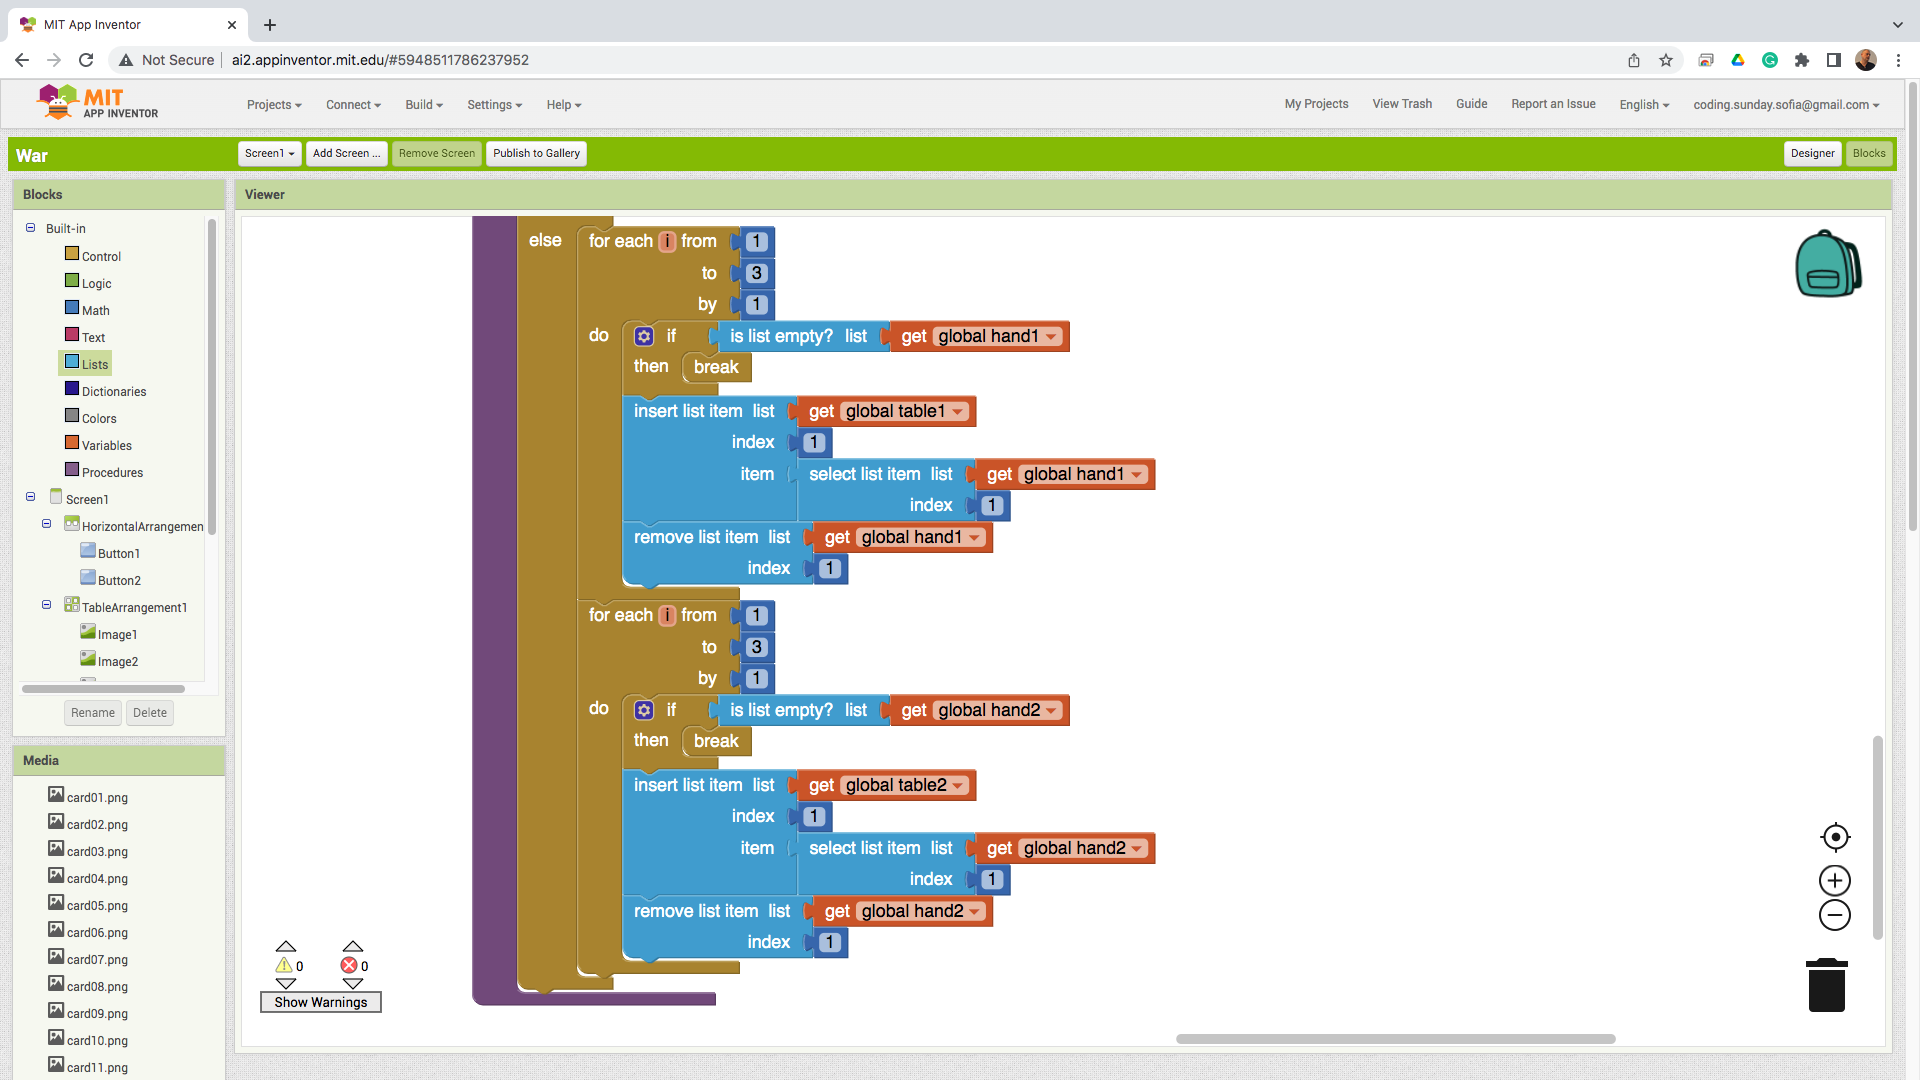
\includegraphics[width=1.0\linewidth,height=0.5\linewidth]{fig100029.png}
   \caption{Removing three cards to the table}
\label{fig100029}
\end{figure}

\section{Publish the project}

The game is made publicly available by publishing it in the "gallery" area (Fig. \ref{fig100030}).

\begin{figure}[H]
   \centering
   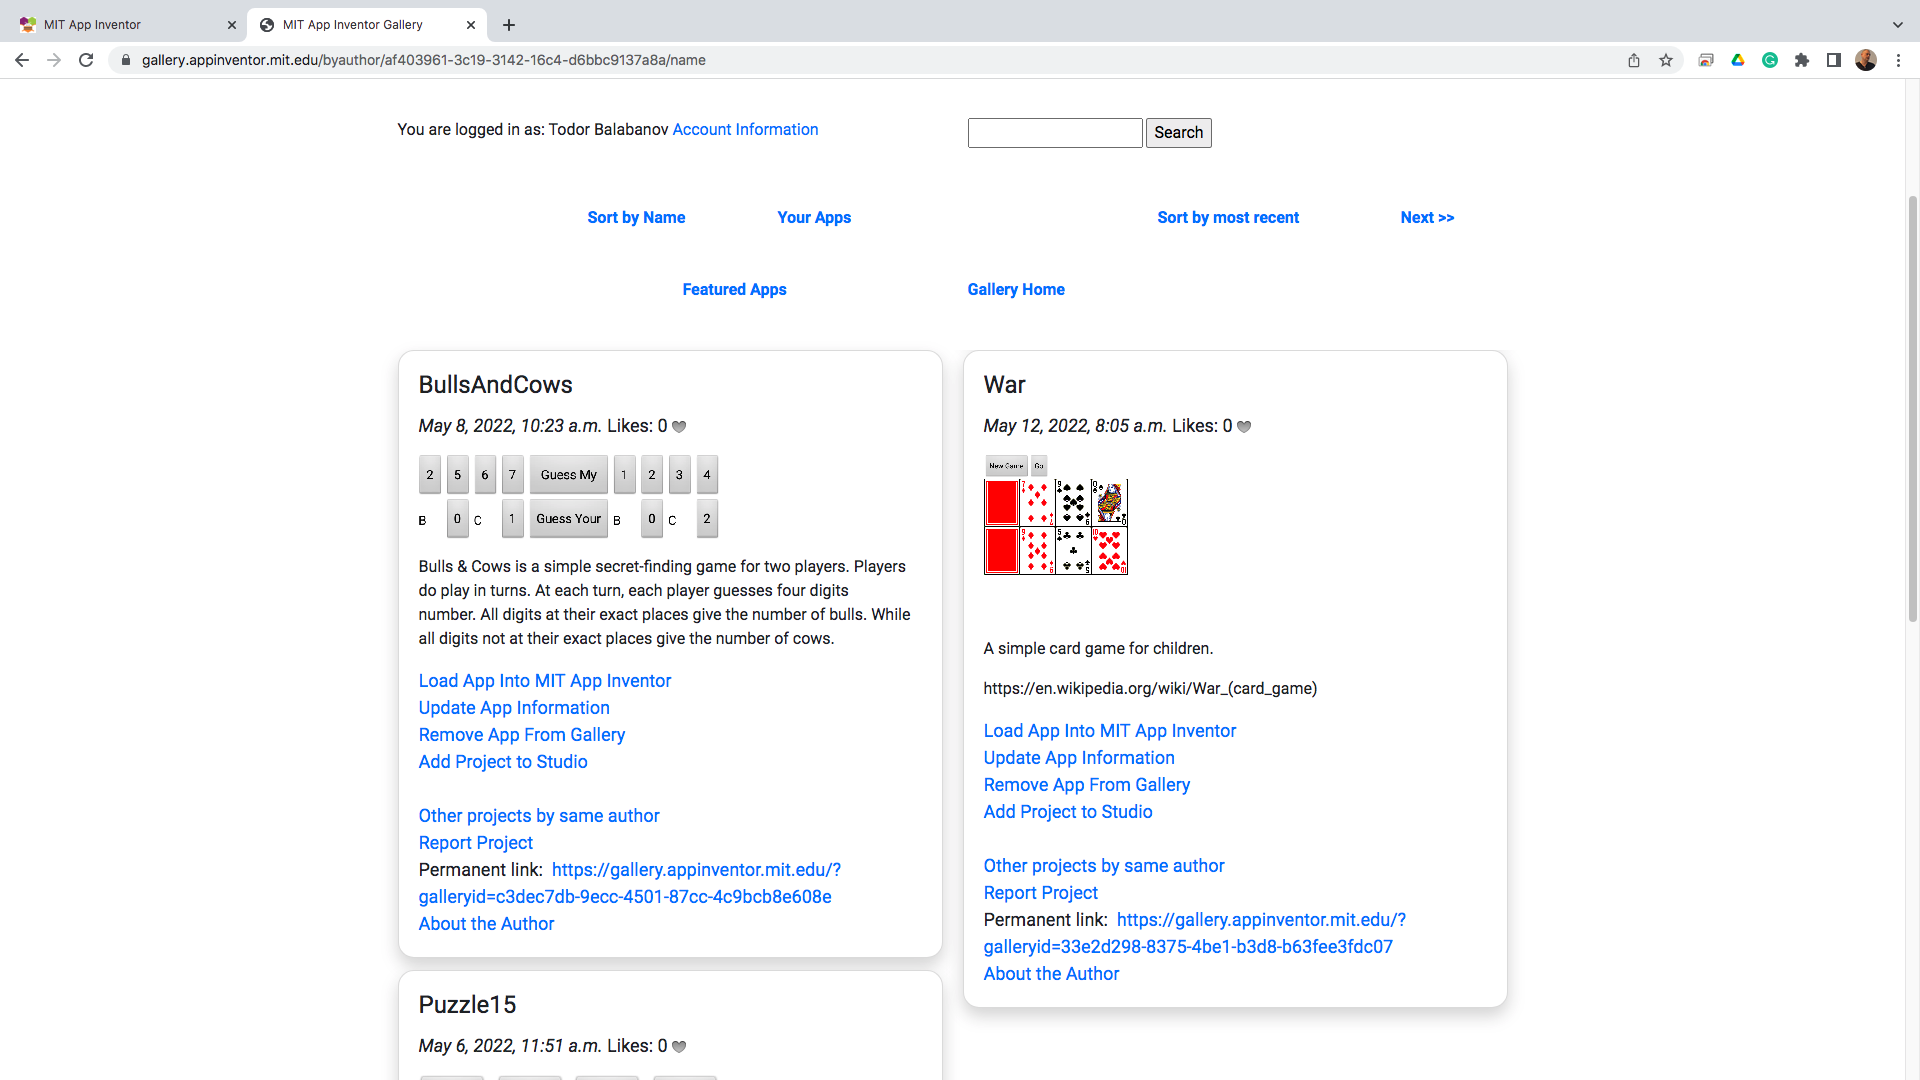
\includegraphics[width=1.0\linewidth,height=0.5\linewidth]{fig100030.png}
   \caption{Publishing the game to the general audience}
\label{fig100030}
\end{figure}

With this, the game takes on its original completeness. Of course, there is still a lot of work to be done to turn it from a hobbyist project into a mass-use software product. First, the visualization of the cards can be improved and give a better account of which player holds how many cards. Help information needs to be included and layout in the form of animations when the cards move. These improvements are beyond the scope of this paper and are left for further exercise by the readers.
